% Railway Digital Twin with Wildlife Safety — academic project report
% College of Engineering, Guindy — Anna University, Chennai - 25
% Course: Embedded Systems and Internet of Things — Team 14
\documentclass[12pt,a4paper]{report}

\usepackage[a4paper,margin=2.6cm,top=2.8cm,bottom=2.8cm]{geometry}
\usepackage[T1]{fontenc}
\usepackage[utf8]{inputenc}
\usepackage{graphicx}
\usepackage{booktabs}
\usepackage{tabularx}
\usepackage{longtable}
\usepackage{multirow}
\usepackage{array}
\usepackage{enumitem}
\usepackage{xcolor}
\usepackage{tikz}
\usetikzlibrary{arrows.meta,positioning,shapes.geometric}
\usepackage{float}
\usepackage{caption}
\usepackage{setspace}
\usepackage{fancyhdr}
\usepackage[hidelinks]{hyperref}
\usepackage{url}

\graphicspath{{figures/}}
\onehalfspacing

\captionsetup{font=small,labelfont=bf}
\setlength{\parskip}{5pt}
\setlength{\parindent}{0pt}

\pagestyle{fancy}
\fancyhf{}
\fancyhead[L]{\small Railway Digital Twin with Wildlife Safety}
\fancyhead[R]{\small\thepage}
\renewcommand{\headrulewidth}{0.4pt}

\begin{document}

% ===================== TITLE PAGE =====================
\begin{titlepage}
\begin{center}

{\large\bfseries COLLEGE OF ENGINEERING, GUINDY}\\[2pt]
{\normalsize\bfseries ANNA UNIVERSITY, CHENNAI -- 25}\\[26pt]

{\Large\bfseries Railway Digital Twin with Wildlife Safety}\\[4pt]
{\normalsize An Educational Simulation Integrating Godot 4, MQTT,\\ a Trusted Node.js Control Plane and ESP32 Edge Sensing}\\[26pt]

{\normalsize\bfseries Submitted in partial fulfillment of the course}\\[2pt]
{\normalsize\bfseries ``Embedded Systems and Internet of Things''}\\[26pt]

% no logo image exists in the repository; omit the emblem rather than fabricate one
{\normalsize\bfseries Submitted By}\\[4pt]
\textbf{Team: 14}\\[10pt]
{\renewcommand{\arraystretch}{1.35}%
\begin{tabular}{r l}
\textbf{Register Number} & \textbf{Name} \\
2023103546 & \; Kathir Kalidass B \\
2023103597 & \; Malini R \\
2023103600 & \; Parthasarathi S \\
2023103714 & \; Paril T \\
\end{tabular}}\\[22pt]

{\normalsize October 2026}

\end{center}
\end{titlepage}

\pagenumbering{roman}
\setcounter{page}{2}

% ===================== ABSTRACT =====================
\chapter*{Abstract}
\addcontentsline{toc}{chapter}{Abstract}

Train--animal collisions remain a persistent operational risk on forested and
rural railway corridors while conventional level-crossing protection offers the
same single mechanism for every kind of intruder. This project develops an
educational \emph{Railway Digital Twin with Wildlife Safety}: a complete,
runnable miniature of a modern wildlife-protected railway line in which the
same event can be observed simultaneously from four cooperating surfaces --- a
three-dimensional twin simulation, a web operations dashboard, a trusted
backend control plane, and an ESP32 edge controller, each communicating over
an authenticated IoT message bus.

The system is built as a staged software stack. \textbf{Godot~4.7} renders a
two-track ``stadium'' railway world (UP and DOWN loops of 1253.98~m and
1228.85~m around a 250~m straight-sided footprint) with an island station,
interlocked crossovers, a wildlife level crossing with boom barriers, carved
river with road and railway bridges, catenary, dynamic signal masts and
Libre-TrainSim-derived Blender train, station, deer and
elephant assets. \textbf{Node.js~22+} with Express and SQLite is the trusted
control plane: the sole publisher of railway commands, state snapshots and
alerts, enforcing bcrypt/JWT authentication, role-based access control
(viewer/operator/admin), command-envelope validation, anti-replay protection
through a persistent SQLite registry, and a full audit trail.
\textbf{Eclipse Mosquitto~2} brokers the machine traffic on
MQTT~TCP~1883/WebSocket~9001 with per-client credentials and least-privilege
topic ACLs. A \textbf{React~18/Vite} dashboard presents live state, per-block
signal aspects, per-train speed control, meet scheduling, wrong-line routing
and hazard evidence badges. An \textbf{ESP32 (Arduino/PlatformIO)} node carries
fail-safe field inputs --- wildlife and sensor-fault pulls, protective outputs,
debounce, SNTP-gated clock truth and non-blocking telemetry. A
\textbf{FastAPI ML microservice} using torchvision's SSDLite MobileNetV3
detector confirms animal sightings from twin-camera frames behind a
two-frame evidence policy.

The wildlife protection chain implements a staged escalation
NONE $\rightarrow$ SUSPECTED (30~km/h limit) $\rightarrow$ CONFIRMED
(0~km/h, STOP/RED) driven by trackside sensor huts, onboard simulated
cameras and ESP32 edge reports, with backend-authoritative hazard fusion,
recovery-latched resets and restrictive fail-safe behaviour on any loss of
communication. Every subsystem is verified by an automated gate ---
42/42 Godot suites, 141/141 backend tests, 8/8 ML tests, 16/16 ESP32 native
tests and a clean web build --- plus live end-to-end scenarios including a
chance-based meet scheduling, an interlocked wrong-line run and the
two-frame camera confirmation chain end-to-end on the live stack. The
system is emphatically a classroom simulation and not certified railway
signalling equipment.

\vspace{6pt}
\noindent\textbf{Keywords:} Digital Twin, Railway Safety, Wildlife, MQTT,
IoT, ESP32, Godot Engine, Node.js, React, Machine Learning
\clearpage
% ===================== TOC / LOF / LOT =====================
\tableofcontents
\clearpage
\listoffigures
\clearpage
\listoftables
\clearpage
%
\pagenumbering{arabic}

% ===================== CHAPTER 1 — INTRODUCTION =====================
\chapter{Introduction}\label{cha:introduction}

\section{Background}

Indian Railways reserves operate through large tracts of forest and open
grassland in which scheduled and unscheduled train paths intersect with
animal movement corridors. Elephants, deer and other wildlife cross
railway formation at grade, and collisions remain a persistent operational
and ecological risk. Conventional protection --- signage, whistle zones and
manual watchmen --- is sparse by design, and a single fixed level-crossing
alarm cannot adapt on its own to \emph{which} animal is ahead, \emph{where}
it is relative to a moving train, or \emph{how much} braking distance the
train still has.

Modern practice addresses this with two converging ideas:

\begin{itemize}
  \item \textbf{Digital twins:} a live virtual replica of a physical asset
        (here, a forest railway line with its trains, signals and crossing)
        that stays synchronised with trusted state and lets operators
        observe, rehearse and reason about operations.
  \item \textbf{Embedded IoT sensing:} low-cost edge devices (here, an
        ESP32 with sensors, protective outputs and a fail-safe state
        machine) at the trackside, publishing machine observations over an
        authenticated message bus rather than treated independently.
\end{itemize}

This project, developed as an educational simulation by Team 14 for the
course \emph{Embedded Systems and Internet of Things}, brings both ideas
together in a system small enough to run on one laptop: a three-dimensional
digital twin of a forest railway loop, a trusted backend control plane, a
role-aware web dashboard, an authenticated MQTT broker, and an ESP32 edge
controller --- all exchanging sensor observations, authority commands,
state snapshots and alerts over well-defined topics.

\section{Objectives}

The objectives of the project are:

\begin{enumerate}
  \item Build a runnable \textbf{3D digital twin} of a double-track forest
        railway --- UP and DOWN loops, an island station with interlocking
        crossovers, a wildlife level crossing with boom barriers, a carved
        river with road and railway bridges, catenary, dynamic signals and
        an LTS-derived Blender asset fleet --- in Godot~4.
  \item Construct a \textbf{trusted control plane} that owns all railway
        authority: a two-train double-track fleet model, per-block signal
        aspects, a fixed-timestep simulation loop, a station-crossover
        interlocking, chance-based meet scheduling, an operator-requestable
        interlocked wrong-line run, and a wildlife-hazard state machine ---
        served over authenticated REST and MQTT.
  \item Enforce \textbf{security end to end}: authenticated users with
        role-based access control, an authenticated MQTT broker with
        per-client topic ACLs, command-envelope validation with
        timestamp freshness and anti-replay protection, and a complete
        audit trail.
  \item Implement \textbf{wildlife sensing and staged protection}: a
        NONE~$\rightarrow$~SUSPECTED~$\rightarrow$~CONFIRMED escalation
        driven by trackside sensor huts, an onboard simulated camera
        detector with analytic occlusion and a quadratic stopping-distance
        model, a backend camera ingest pipeline with two-frame evidence
        confirmation, and ML-assisted animal detection through a FastAPI
        microservice.
  \item Implement an \textbf{ESP32 edge node} with restrictive fail-safe
        outputs, debounced local inputs, SNTP-gated clock truth,
        non-blocking telemetry and edge-triggered wildlife alerts ---
        validated natively and in the Wokwi cloud simulator.
  \item Provide a \textbf{role-aware dashboard} for viewer, operator and
        admin users with live state, per-block aspects, per-train speed
        control, route/meet/wrong-line panels and hazard evidence badges.
  \item Verify the whole stack continuously with an automated
        multi-surface test gate and documented live end-to-end scenarios.
\end{enumerate}

\section{Scope and safety boundary}\label{sec:scope}

Two scope statements are as important as the features themselves:

\begin{itemize}
  \item \textbf{Educational simulation only.} The system is a classroom
        digital-twin simulation, \emph{not} railway safety equipment. It
        must never be connected to real signalling, trains or operational
        infrastructure. Simulated ``stopping distance'' is a visualization
        estimate only and does not model certified train dynamics,
        gradients, adhesion or real braking curves.
  \item \textbf{Physical hardware status.} The ESP32 path was verified
        through the Wokwi cloud simulator (via a Pinggy tunnel to the
        local authenticated broker). The physical-hardware checklist items
        in the Stage~D plan remain \emph{not run}: real instruments were
        not connected. The report is explicit wherever this applies.
\end{itemize}

Within those boundaries, every subsystem --- backend, twin, dashboard,
firmware and ML service --- is fully implemented and gated by automated
tests (Chapter~\ref{cha:features}, Appendix~\ref{cha:appendix-gates}).

\section{Phased implementation outline}

The system was built in recorded, gated stages (dates from
\texttt{docs/porting/acceptance.md}):

\begin{itemize}
  \item \textbf{Stage A (backend foundation)} --- Express + JWT/RBAC,
        SQLite audit and anti-replay registry, two-zone state machine,
        backend-authoritative MQTT, broker auth and ACLs
        (2026-10-18/19).
  \item \textbf{Stage A2 (block signalling)} --- per-block aspects and
        retained signals (2026-10-19).
  \item \textbf{Stage B (dashboard)} --- login, role-aware REST controls,
        WebSocket live updates, audit feed (2026-10-19).
  \item \textbf{Stage C (Godot twin)} --- vendored MQTT bridge, procedural
        world, train/wildlife animation, brakes, signals, cameras;
        porting Libre-TrainSim (LTS) Blender assets (2026-10-19/20).
  \item \textbf{Stage D (ESP32 / Wokwi)} --- per-client credentials,
        device-scoped topics, fail-safe outputs, cloud simulation through
        a tunnel (2026-10-19/20).
  \item \textbf{Stage E (integrated delivery)} --- Docker/environment
        setup, scenario scripts and the formal acceptance record
        (2026-10-22).
  \item \textbf{Stage 2A--2G (double-track phase)} --- a two-train UP/DOWN
        fleet, ten blocks with aspects, station island and crossovers
        (2A), the double-track world (2B--2C), backend lives and camera
        fleet (2A--2D), meet/pass scenarios (2E, 2G), and distributed
        wildlife sensing with an onboard detector (2F) (2026-10-21/22).
  \item \textbf{Stadium evolution --- Phases 1--3} --- both loops reshaped
        as one 250~m straight-sided shared stadium footprint with opposite
        operational chainage (2026-10-22), an interlocked operator
        wrong-line run with an opposing-train hold (2026-10-23), and the
        staged camera/ML/near-animal confirmation chain with two-frame
        evidence (2026-10-23).
\end{itemize}

\section{Organisation of the report}

Chapter~2 states requirements. Chapter~3 describes the system architecture
and end-to-end workflow. Chapter~4 documents tools and technology.
Chapter~5 covers hardware, peripherals and the simulation stack.
Chapter~6 details the digital twin world. Chapter~7 documents the
dashboards. Chapter~8 lists every implemented feature and function with
its verification evidence. Chapter~9 presents results, limitation and
conclusion. Appendices collect the access-control matrix, the complete
test-gate record and run instructions. Reproduced simulation screenshots
appear in Figures~\ref{fig:overview}--\ref{fig:cameraconfirm} and the
figures referenced from Chapters~5--8.

% ============ CHAPTER 2 — SYSTEM REQUIREMENTS AND PHASES ============
\chapter{System Requirements and Phases}\label{cha:requirements}

\section{Functional requirements}

\begin{longtable}{>{\raggedright}p{0.8cm} >{\raggedright\arraybackslash}p{10.6cm} l}
\caption{Functional requirements and delivery phase}\label{tab:functional}\\
\toprule
\textbf{S.No} & \textbf{Requirement} & \textbf{Phase} \\
\midrule
\endfirsthead
\caption[]{(continued)}\\
\toprule
\textbf{S.No} & \textbf{Requirement} & \textbf{Phase} \\
\midrule
\endhead
FR-1 & Authenticate users (bcrypt passwords, JWT sessions) with three roles: viewer (monitor), operator (control), admin (audit inspection). & A \\
FR-2 & Validate every command envelope against schema with $\pm$5\,min timestamp freshness and reject replays through a persistent SQLite \texttt{processed\_requests} registry. & A \\
FR-3 & Record an audit row (actor, role, zone, action, result, timestamp) for every control attempt --- accepted, rejected or forbidden. & A \\
FR-4 & On MQTT disconnect apply the restrictive \texttt{COMM\_LOST} fail-safe; on reconnect publish the retained state snapshot to reconcile clients. & A \\
FR-5 & Be the sole publisher of commands, state snapshots, alerts and signals on MQTT with per-client topic ACLs. & A \\
FR-6 & Reject a reset while a wildlife hazard or sensor fault is active (operator must clear and then explicitly reset). & A \\
FR-7 & Model a two-train (T1 UP, T3 DOWN) double-track fleet with ten blocks, per-block signal aspects, occupancy safety and a fixed-timestep simulation loop. & 2A \\
FR-8 & Provide a station-crossover interlock: one route at a time, hazard/occupancy checks, 409 on conflicts, automatic release. & 2A, 2G \\
FR-9 & Run chance-based meet scheduling from a seeded PRNG: hold the slower train at the station, execute the crossover as a proper route, reproduce history for identical seeds. & 2G \\
FR-10 & Let an operator request an interlocked wrong-line run (UP$\rightarrow$DOWN at crossover A, return at B) while the opposing train is held automatically inside braking distance; phases APPROACH~$\rightarrow$~CROSS\_ENTRY~$\rightarrow$~WRONG\_LINE~$\rightarrow$~CROSS\_EXIT~$\rightarrow$~CLEARANCE~$\rightarrow$~DONE. & Stadium P2 \\
FR-11 & Operate distributed trackside wildlife huts --- UP-S0..UP-S4 and DOWN-S0..DOWN-S4, i.e.\ ten huts with 75\,m overlapping radius --- publishing observations used as \emph{trackside} evidence. & 2F \\
FR-12 & Provide onboard simulated-ML camera detection (forward cone vision, $\pm$25$^\circ$/10$^\circ$, 200\,m range, analytic occlusion against terrain, trunks and bridge decks) as \emph{onboard} evidence with zero-latency local braking. & 2F \\
FR-13 & Accept camera frames over authenticated HTTP (bearer token, \texttt{X-Captured-At} freshness, duplicate-id suppression), validate blocks and line, run the ML detector, and confirm a hazard only on \emph{two} frames. & Stadium P3 \\
FR-14 & Implement staged hazard escalation: trackside-only suspicion caps the approaching train at 30\,km/h and shows YELLOW; camera confirmation stops the train (0\,km/h) and shows RED; clearing never downgrades a confirmed block; reset is required after hazard clear. & Stadium P3 \\
FR-15 & Deliver ESP32 edge alerts (\texttt{WILDLIFE\_NEAR}, \texttt{WILDLIFE\_DETECTED}, \texttt{WILDLIFE\_CLEARED}) to the edge node and require operator re-arm (RESET) through the dashboard. & Stadium P3 \\
FR-16 & Render the twin: stadium double-track world, island station, interlocked crossovers, two-track level crossing, river with bridges, catenary, dynamic signals, barriers, cameras and HUD. & C, 2B--2E, Stadium P1 \\
FR-17 & Provide the dashboard: login, live state via WebSocket, train cards with speed control, block-aspect diagram, evidence badges, meet card, wrong-line panel, camera health. & B, 2E--2G, P3 \\
FR-18 & Publish ESP32 telemetry with SNTP-validated UTC time; reject stale, malformed, duplicate or wrong-zone telemetry at the backend and mark clock-invalid telemetry before it is sent. & D \\
\bottomrule
\end{longtable}

\section{Non-functional requirements}

\begin{longtable}{>{\raggedright}p{0.8cm} >{\raggedright\arraybackslash}p{10.7cm} l}
\caption{Non-functional requirements}\label{tab:nonfunctional}\\
\toprule
\textbf{S.No} & \textbf{Requirement} & \textbf{Where enforced} \\
\midrule
\endfirsthead
\caption[]{(continued)}\\
\toprule
\textbf{S.No} & \textbf{Requirement} & \textbf{Where enforced} \\
\midrule
\endhead
NFR-1 & \textbf{Security --- least privilege:} every MQTT client authenticates; per-client ACLs allow the dashboard read-only access, Godot telemetry-publish-only on its zones, and the backend full control topics. & \texttt{mosquitto/acl\_file}, broker ACL tests \\
NFR-2 & \textbf{Fail-safety:} every output is restrictive at startup, on communication loss, on fresh-context loss, and for active local hazard/fault inputs; local inputs cannot be cleared remotely. & backend state machine, ESP32 \texttt{output\_logic.h} \\
NFR-3 & \textbf{Anti-replay:} accepted REST control IDs/timestamps persists in SQLite; stale, duplicated or schema-invalid envelopes are rejected. & \texttt{command\_tracker.js}/SQLite \\
NFR-4 & \textbf{Auditability:} every control or route attempt recorded in SQLite regardless of outcome; admin-only inspection. & \texttt{audit.js} \\
NFR-5 & \textbf{Reproducibility:} seeded PRNG (meet scheduler and wildlife director) gives identical histories for identical seeds; same command must produce the same state. & \texttt{rng.js}, \texttt{meets.js} \\
NFR-6 & \textbf{Performance:} backend snapshot publish loop of 2\,Hz; train-speed updates smooth at the twin; live state and camera ingest stay within documented limits (camera ingest $>$5\,fps rate-limited, 413 on oversize). & \texttt{loop.js}, camera ingest \\
NFR-7 & \textbf{Testability:} every surface gated by automated tests; the gate must exit non-zero on any failure and be re-runnable headless. & \texttt{verify-all.sh}, test suites \\
NFR-8 & \textbf{Educational honesty:} stopping distance is a visualization estimate; not certified signalling; the system never touches real railway infrastructure. & README, presentation \\
NFR-9 & \textbf{Compose-neutral developer path:} one script \texttt{dev-up.sh} to stand up the stack, reset the demo, generate broker credentials. & scripts/ \\
\bottomrule
\end{longtable}

\section{Hardware requirements}

\begin{longtable}{>{\raggedright}p{4.5cm} >{\raggedright\arraybackslash}p{9.0cm}}
\caption{Hardware requirements}\label{tab:hardware}\\
\toprule
\textbf{Item} & \textbf{Specification} \\
\midrule
Development host & x86-64 PC with Linux or WSL2; mouse/keyboard for the twin. GPU useful but not required (Mesa llvmpipe software rendering is supported for headless verification) \\
Docker engine & Docker Engine with Compose v2; no ``docker desktop'' required \\
ESP32 devkit v1 & Optional for the edge-node path (equivalently simulated on Wokwi); Wi-Fi capable, MCP UART 115\,200 \\
Sensors/indicators & Green/red LEDs, buzzer, pushbuttons (wildlife, fault), SSD1306 OLED, servo (all simulated in Wokwi); telemetry needs network reachability to the broker \\
Cameras & None physical; twin camera feeds are simulated render outputs consumed by the ML microservice \\
\bottomrule
\end{longtable}

\section{Software requirements}

\begin{longtable}{>{\raggedright}p{4.5cm} >{\raggedright\arraybackslash}p{9.0cm}}
\caption{Software requirements}\label{tab:software}\\
\toprule
\textbf{Layer} & \textbf{Tool / version} \\
\midrule
OS & Ubuntu 24.04 LTS (WSL2 permissible) \\
Container runtime & Docker Engine + Compose; images \texttt{eclipse-mosquitto:2}, Node base image \\
Control plane & Node.js 22+ (runtime 24 of the verification host), Express 4.21, better-sqlite3 13, bcryptjs 3, jsonwebtoken 9, mqtt.js 5.16 \\
Broker & Eclipse Mosquitto 2 --- TCP 1883, WebSocket 9001, \texttt{allow\_anonymous false} \\
Dashboard & React 18.3.1, Vite 6, TypeScript 5.7, \texttt{lucide-react} \\
Twin engine & Godot 4.7.2 (GL compatibility for headless render) \\
Firmware & PlatformIO (\texttt{espressif32}, \texttt{arduinoframework}), PubSubClient 2.8, ArduinoJson 7, ESP32Servo, Adafruit SSD1306/GFX \\
Edge simulation & Wokwi CLI v0.29.0; tunnel via Pinggy raw TCP \\
ML microservice & Python, FastAPI 0.135.1, uvicorn, torch 2.10.0, torchvision 0.25.0 (SSDLite320 MobileNetV3, COCO animal classes), Pillow, NumPy \\
Quality & Node built-in test runner (backend), Godot test harness (42 suites), Pytest (ML), PlatformIO Unity (ESP32 native), Vite/TypeScript build check \\
\bottomrule
\end{longtable}

\section{Phase-to-gate mapping}

\begin{longtable}{>{\raggedright}p{1.3cm} >{\raggedright\arraybackslash}p{6.2cm} >{\raggedright\arraybackslash}p{5.6cm}}
\caption{Delivery phases vs verification evidence}\label{tab:phasemap}\\
\toprule
\textbf{Phase} & \textbf{Deliverable} & \textbf{Evidence} \\
\midrule
A / A2 & Trusted backend, two-zone and later block signalling & \texttt{state.test.js}, \texttt{signalling.test.js}, \texttt{broker\_acl.test.js} \\
B & Authenticated role-aware dashboard & Rest API tests, web build \\
C & Godot twin with LTS-derived assets & 42 Godot suites incl.\ \texttt{test\_real\_assets} \\
D & ESP32 fail-safe edge node & 16 native Unity cases + Wokwi scenario \\
E & Integrated stack + formal acceptance record & \texttt{docs/porting/acceptance.md} \\
2A--2C & Double-track fleet, world, crossovers & \texttt{signalling/routes/meets} suites, Godot track registry suites \\
2E--2G & Meet/pass and chance-based meets with interlocking & \texttt{test\_meet\_scenario}, \texttt{meets.test.js}, \texttt{rng.test.js} \\
2F & Distributed wildlife sensing + onboard detector + braking model & \texttt{test\_sensor\_huts}, \texttt{test\_onboard\_detector}, \texttt{test\_onboard\_braking} \\
Stadium P1--P3 & Shared stadium geometry, wrong-line run, camera/ML/near-animal chain & \texttt{test\_stadium\_track}, \texttt{wrong\_line*.test.js}, \texttt{near\_animal.test.js}, \texttt{camera.test.js} \\
\bottomrule
\end{longtable}

% ============ CHAPTER 3 — ARCHITECTURE AND WORKFLOW ============
\chapter{System Architecture and Workflow}\label{cha:architecture}

\section{Architecture overview}

The system is organised around one principle: \textbf{one trusted control
plane, many observing/edge clients}. The Node.js backend is the single
authority for train commands, block aspects, routes, meets, hazards and
alerts; every other component either publishes observations (Godot twin,
ESP32) or consumes authoritative state (dashboard, twin, ESP32). Figure~%
\ref{fig:arch-block} shows the five subsystems and their interfaces.

\begin{figure}[H]
\centering
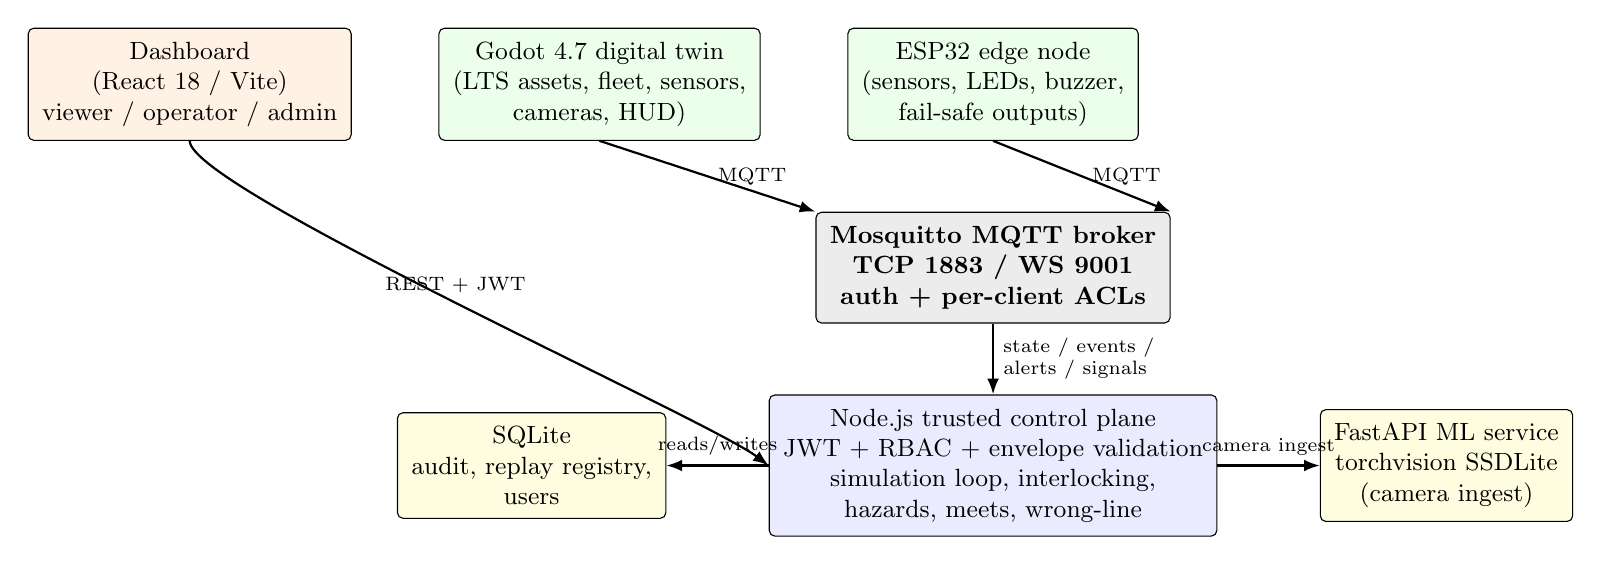
\begin{tikzpicture}[
  node distance=9mm and 11mm,
  box/.style={draw, rounded corners=2pt, align=center, inner sep=5pt, font=\small},
  auth/.style={box, fill=blue!8},
  edge/.style={box, fill=green!8},
  view/.style={box, fill=orange!10},
  store/.style={box, fill=yellow!12},
  bus/.style={box, fill=gray!15, font=\small\bfseries},
  line/.style={-{Latex[length=2mm]}, thick},
]
  % clients row
  \node[view] (dash) {Dashboard\\(React 18 / Vite)\\viewer / operator / admin};
  \node[edge, right=of dash] (twin) {Godot 4.7 digital twin\\(LTS assets, fleet, sensors,\\ cameras, HUD)};
  \node[edge, right=of twin] (esp) {ESP32 edge node\\(sensors, LEDs, buzzer,\\ fail-safe outputs)};
  % broker middle
  \node[bus, below=of esp] (broker) {Mosquitto MQTT broker\\TCP 1883 / WS 9001\\auth + per-client ACLs};
  % backend bottom
  \node[auth, below=of broker] (backend) {Node.js trusted control plane\\JWT + RBAC + envelope validation\\simulation loop, interlocking,\\hazards, meets, wrong-line};
  % stores side
  \node[store, left=of backend, xshift=-2mm] (sql) {SQLite\\audit, replay registry,\\users};
  \node[store, right=of backend, xshift=2mm] (ml) {FastAPI ML service\\torchvision SSDLite\\(camera ingest)};
  % REST links
  \draw[line] (dash.south) .. controls +(0,-0.6) and +(-0.8,0.6) .. node[above, font=\scriptsize]{REST + JWT} (backend.west);
  \draw[line] (backend) -- node[above, font=\scriptsize]{reads/writes} (sql);
  \draw[line] (backend) -- node[above, font=\scriptsize]{camera ingest} (ml);
  % links through broker
  \draw[line] (twin.south) -- node[right, font=\scriptsize]{MQTT} (broker.north west);
  \draw[line] (esp.south) -- node[right, font=\scriptsize]{MQTT} (broker.north east);
  \draw[line] (broker) -- node[right, align=left, font=\scriptsize]{state / events /\\alerts / signals} (backend);
\end{tikzpicture}
\caption{System block diagram: one trusted control plane, many clients.}
\label{fig:arch-block}
\end{figure}

The four cooperating surfaces are:

\begin{enumerate}
  \item \textbf{Mosquitto broker} (TCP~1883, WebSocket~9001) with
        \texttt{allow\_anonymous false}; credentials are generated by
        \texttt{scripts/mosquitto\_setup.sh} from local environment
        variables; per-client ACLs in \texttt{mosquitto/acl\_file} enforce
        the topic contract (Appendix~\ref{cha:appendix-acl}).
  \item \textbf{Node.js backend} --- authenticates users with bcrypt and
        JWT, enforces RBAC (viewer/operator/admin), validates command
        envelopes, blocks replays through a persistent SQLite
        \texttt{processed\_requests} registry, writes an audit trail for
        every control attempt, runs the two-train simulation loop, owns
        block signalling, crossover interlocking, meet scheduling, the
        wrong-line state machine and the wildlife-hazard fusion --- and is
        the sole MQTT publisher of commands, state, alerts and signals.
  \item \textbf{Godot 4.7 twin} --- full-scale double-track world with the
        LTS-derived asset fleet (Chapter~\ref{cha:twin}); reconciles
        backend state into train targets and signals, publishes track
        telemetry and wildlife evidence; also executes its own local
        fail-safe limit that can only \emph{tighten} the backend target.
  \item \textbf{React dashboard} --- authenticated REST for control,
        MQTT-over-WebSocket for live updates; read-only on MQTT.
  \item \textbf{ESP32 node} --- authenticated IoT client restricted to
        telemetry publish + command subscribe on its own topics.
\end{enumerate}

\section{Data flow and message contract}

Figure~\ref{fig:dataflow} traces the canonical control and observation
paths. Two flows are deliberately asymmetric:

\begin{itemize}
  \item \textbf{Control flows REST} (dashboard $\rightarrow$ backend only)
        so every command crosses the authenticated, audited, anti-replayed
        boundary once.
  \item \textbf{State flows MQTT} (backend $\rightarrow$ all clients,
        retained) so any late joiner sees the current truth without
        polling, and a lost client resynchronises from the retained
        snapshot on reconnect.
\end{itemize}

\begin{figure}[H]
\centering
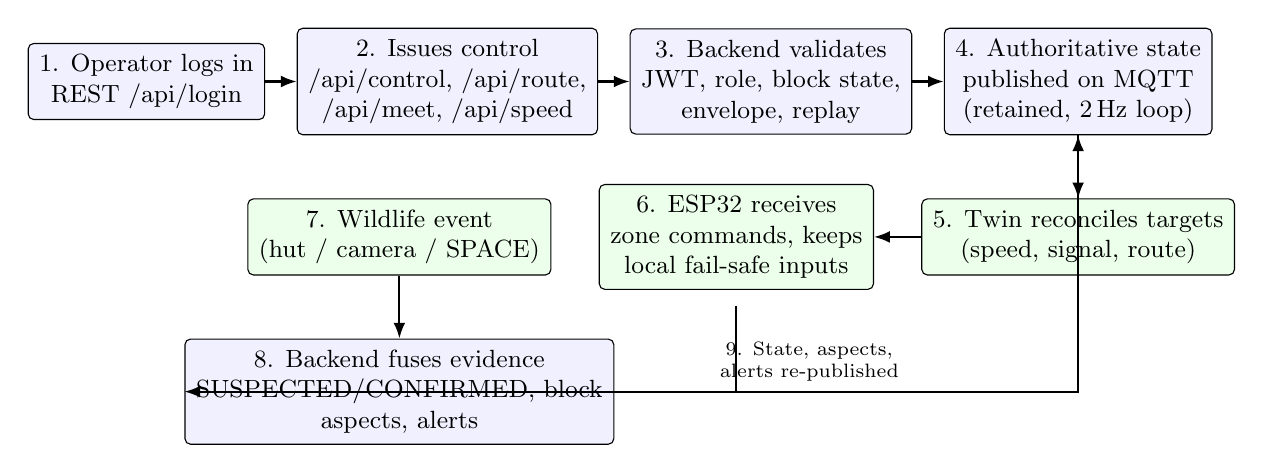
\begin{tikzpicture}[
  font=\small,
  every node/.style={align=center},
  wstep/.style={draw, rounded corners=2pt, minimum height=8mm, inner sep=4pt, fill=blue!6},
  obs/.style={wstep, fill=green!8},
  line/.style={-{Latex[length=2mm]}, thick},
]
  \node[wstep] (a) {1. Operator logs in\\REST /api/login};
  \node[wstep, right=4mm of a] (b) {2. Issues control\\/api/control, /api/route,\\/api/meet, /api/speed};
  \node[wstep, right=4mm of b] (c) {3. Backend validates\\JWT, role, block state,\\envelope, replay};
  \node[wstep, right=4mm of c] (d) {4. Authoritative state\\published on MQTT\\(retained, 2\,Hz loop)};
  \node[obs, below=8mm of d] (e) {5. Twin reconciles targets\\(speed, signal, route)};
  \node[obs, left=6mm of e] (f) {6. ESP32 receives\\zone commands, keeps\\local fail-safe inputs};
  \node[obs, left=6mm of f] (g) {7. Wildlife event\\(hut / camera / SPACE)};
  \node[wstep, below=8mm of g] (h) {8. Backend fuses evidence\\SUSPECTED/CONFIRMED, block\\aspects, alerts};
  \draw[line] (a) -- (b);
  \draw[line] (b) -- (c);
  \draw[line] (c) -- (d);
  \draw[line] (d) -- (e);
  \draw[line] (e) -- (f);
  \draw[line] (f.south) ++(0,-2mm) |- (h.west);
  \draw[line] (g) -- (h);
  \draw[line] (h.east) ++(2mm,0) -| node[pos=0.2, above, font=\scriptsize]{9. State, aspects,\\alerts re-published} (d.south);
\end{tikzpicture}
\caption{End-to-end workflow: control (steps 1--4) and wildlife observation
(steps 5--9) as one closed loop.}
\label{fig:dataflow}
\end{figure}

\section{Backend internal architecture}

The backend is composed of small single-responsibility modules
(\texttt{backend/src/}) composing a fixed-timestep simulation loop
(\texttt{loop.js}) that ticks authoritative state and publishes snapshots
at 2\,Hz once the broker connection is up:

\begin{itemize}
  \item \texttt{config.js} --- fleet, blocks, lines, station, crossovers,
        meet parameters and wrong-line hold points (UP 1253.9822\,m,
        DOWN 1228.8495\,m lengths).
  \item \texttt{state.js} / \texttt{simulation.js} --- authoritative
        trains T1 (UP, clockwise) and T3 (DOWN, anticlockwise), block
        occupancy, per-train speed dynamics and dwell logic.
  \item \texttt{signalling.js} / \texttt{routes.js} --- per-block aspects,
        retained \texttt{railway/signal/\{block\}} topics, station
        crossover interlocking and route lifecycle.
  \item \texttt{meets.js} / \texttt{rng.js} --- seeded chance-based meet
        scheduler and its deterministic PRNG.
  \item \texttt{wrong\_line.js} --- the operator-requested wrong-line
        run: APPROACH $\rightarrow$ CROSS\_ENTRY $\rightarrow$ WRONG\_LINE
        $\rightarrow$ CROSS\_EXIT $\rightarrow$ CLEARANCE $\rightarrow$ DONE
        with automated opposing-train hold inside braking distance.
  \item \texttt{wildlife\_commands.js} / \texttt{ingest.js} /
        \texttt{ml.js} --- trackside and onboard evidence fusion, camera
        ingest (bearer token, \texttt{X-Captured-At}, duplicate-id,
        rate and size limits) and ML service calls.
  \item \texttt{auth.js} / \texttt{rbac.js} / \texttt{replay.js} /
        \texttt{audit.js} / \texttt{db.js} --- JWT authentication, role
        checks, replay registry and audit logging backed by SQLite.
  \item \texttt{bus.js} / \texttt{mqtt.js} / \texttt{events.js} ---
        MQTT connection, retained topic publication, WebSocket-ready
        event stream for the dashboard.
  \item \texttt{geometry.js} --- shared UP/DOWN operational vs physical
        chainage conversion used by holds, huts and cameras.
\end{itemize}

\section{Failure handling and fail-safety}

Three deliberate, test-verified behaviours define the safety posture
(Section~\ref{sec:features-safety}):

\begin{itemize}
  \item \textbf{Restrictive fail-safe:} on MQTT loss the backend flags a
        restrictive state; the twin enforces a local limit; the ESP32 is
        restrictive at boot, during loss of fresh backend context, and
        for any active local hazard/fault input. Local inputs are
        debounced and can never be overridden remotely.
  \item \textbf{Recovery latch:} clearing a hazard is never enough; the
        backend latches \texttt{RECOVERY\_REQUIRED} until an authorised
        operator/admin issues RESET with healthy sensors and no active
        hazard. RESET is further rejected while hazards or faults are
        active (per \texttt{IMPLEMENTATION.md}).
  \item \textbf{No command/telemetry replay:} envelopes carry timestamps
        (validated within $\pm$5\,min); IDs deduplicated in SQLite;
        ESP32 telemetry is non-retained, and stale, malformed,
        duplicate or wrong-zone telemetry is rejected. Firmware does not
        queue old telemetry or commands for replay after reconnect.
\end{itemize}

\section{Topic contract summary}

The complete per-client publish/subscribe matrix is in
Appendix~\ref{cha:appendix-acl}. The contract's essence:

\begin{itemize}
  \item backend publishes \texttt{railway/state}, \texttt{railway/events},
        \texttt{railway/alerts}, \texttt{railway/zone*/signal},
        \texttt{railway/commands/*}, \texttt{railway/speed/*},
        \texttt{railway/security/events}, \texttt{railway/wildlife},
        \texttt{railway/signal/\{block\}} (retained);
  \item godot publishes telemetry and wildlife observations for its
        zones; subscribes to commands, speeds, signals and state;
  \item dashboard subscribes to state, events and alerts --- and
        publishes nothing;
  \item esp32 publishes only \texttt{railway/telemetry/esp32}
        (non-retained) and subscribes to \texttt{railway/commands/esp32}.
\end{itemize}

Captured figures of the twin surfaces these chapters describe are in
Figures~\ref{fig:overview}--\ref{fig:wronglineafter}.

% ============ CHAPTER 4 — TOOLS AND TECHNOLOGY ============
\chapter{Tools and Technology}\label{cha:tools}

\section{Technology stack at a glance}

\begin{longtable}{>{\raggedright}p{2.4cm} >{\raggedright\arraybackslash}p{4.6cm} >{\raggedright\arraybackslash}p{8.4cm}}
\caption{Complete technology stack}\label{tab:stacksummary}\\
\toprule
\textbf{Layer} & \textbf{Technology} & \textbf{Role in the system} \\
\midrule
\endfirsthead
\caption[]{(continued)}\\
\toprule
\textbf{Layer} & \textbf{Technology} & \textbf{Role} \\
\midrule
\endhead
Unity of authority & Node.js 22+ with Express 4 & Trusted control plane: auth, RBAC, simulation, interlocking, hazards, audit \\
Data store & SQLite (better-sqlite3 13) & Persistent users, audit rows, anti-replay registry; WAL-mode SQLite file inside a Docker volume \\
Live bus & Eclipse Mosquitto 2 (MQTT 3.1.1) & Authenticated pub/sub bus for all machine traffic over TCP 1883 / WS 9001 \\
Twin & Godot 4.7.2 & Full 3D digital twin scene, physics-free kinematic fleet, cameras, HUD \\
Assets & Blender exports from Libre-TrainSim (LTS) & Train consist GLBs, station modules, deer/elephant, scenery fleet \\
Dashboard & React 18.3.1 + Vite 6 + TypeScript 5.7 & Auth web console with live state and controls \\
Edge node & Arduino framework on ESP32 devkit v1 via PlatformIO & Field sensing, protective outputs, SNTP-gated telemetry \\
Edge simulation & Wokwi (diagram.json, wokwi.toml) + Wokwi CLI v0.29.0 & Cloud-compile and scenario-run without hardware \\
Tunnel & Pinggy raw TCP (\texttt{scripts/wokwi-tunnel.sh}) & Exposes local authenticated broker to the cloud Wokwi session \\
ML service & Python + FastAPI 0.135.1, torch 2.10, torchvision 0.25 & Animal detection (SSDLite320 MobileNetV3, COCO animal classes) over HTTP \\
Verification & Node test runner, Godot test harness (42 suites), Pytest, PlatformIO + Unity (native) & Continuous automated gate across all four surfaces \\
DevOps & Docker Compose, bash scripts & One-command stack bring-up (\texttt{dev-up.sh}) and full gate (\texttt{verify-all.sh}) \\
\bottomrule
\end{longtable}

\section{Backend stack}

\begin{itemize}
  \item \textbf{Node.js 22+} chosen for the built-in test runner, first-class
        \texttt{--env-file-if-exists} startup and the mature MQTT/SQL
        ecosystem on one trusted process.
  \item \textbf{Express 4.21} REST control surface: \texttt{/api/login},
        \texttt{/api/control}, \texttt{/api/route}, \texttt{/api/meet},
        \texttt{/api/speed}, \texttt{/api/wrong-line}, \texttt{/api/camera},
        \texttt{/api/health} --- each with RBAC, envelope validation and
        audit semantics (Chapter~\ref{cha:features}).
  \item \textbf{better-sqlite3 13} embedded database in WAL mode for low
        latency audit and replay persistence; lives in a named Docker
        volume so state survives restarts.
  \item \textbf{bcryptjs 3} password hashing for seed users;
        \textbf{jsonwebtoken 9} for short-lived JWT issuance.
  \item \textbf{mqtt.js 5.16} for both MQTT publishing (state, events,
        alerts, signals, commands, speed) and subscription.
  \item \textbf{Node built-in test runner} for the 141-test suite executed
        with \texttt{--test --test-force-exit}; the MQTT e2e subset runs
        against an isolated Mosquitto container on port 1884 when the
        host broker occupies 1883.
\end{itemize}

\section{Broker and communication}

\begin{itemize}
  \item \textbf{MQTT} chosen as the machine bus: quality-of-service
        semantics (QoS 1 for commands), \emph{retained} messages for state
        and signals (a late joiner instantly sees current truth), topic
        hierarchy as identity, and per-client ACLs as authorization.
  \item \textbf{Mosquitto 2} configured with
        \texttt{allow\_anonymous false}; the password file is produced by
        \texttt{scripts/mosquitto\_setup.sh} from \texttt{.env}
        variables; ACLs restrict clients to the exact topic set listed in
        Appendix~\ref{cha:appendix-acl}.
  \item \textbf{WebSocket listener 9001} serves browser clients so the
        dashboard never needs raw TCP.
  \item Version note: MQTT retained-state design intentionally avoids
        bespoke discovery mechanisms, simplifying the ESP32 client
        (\texttt{PubSubClient}) which supports MQTT 3.1.1.
\end{itemize}

\section{Dashboard stack}

\begin{itemize}
  \item \textbf{React 18} single page application with lucide-react icons;
        builds via \textbf{Vite 6} with a TypeScript gate
        (\texttt{tsc --noEmit}) so type errors fail the web build.
  \item Login flow POSTs to \texttt{/api/login} and stores the JWT in
        memory; subsequent REST calls carry \texttt{Authorization};
        live updates arrive over WebSocket from the backend event stream.
  \item Panels implemented: role-aware header, signal-aspect block
        diagram with CAM/HUT evidence badges, per-train speed control,
        station route card, meet card (seed, phase, countdown), wrong-line
        operator panel with eligibility and cancel, camera health/staged
        hazard panel, and an admin-only audit feed.
\end{itemize}

\section{Twin engine and asset pipeline}

\begin{itemize}
  \item \textbf{Godot 4.7.2} with the \texttt{gl\_compatibility} renderer,
        which keeps the twin runable both locally on GPUs and headless
        under \texttt{xvfb-run} with Mesa llvmpipe software rendering ---
        the mode used for the automated captures used in this report.
  \item \textbf{Libre-TrainSim (LTS) asset port:} the Blender host files
        (\texttt{tools/export\_lts\_assets.py}) export the LTS train
        consist, station modules and scenery to GLB/JSON manifests
        (\texttt{godot/assets.manifest.json}); \texttt{test\_real\_assets}
        proves the tracked GLBs actually replace the procedural fallbacks.
  \item \textbf{Vendored MQTT addon} (\texttt{godot/addons/godot-mqtt})
        plus the LTS runtime addon bridge the twin to the broker with
        backoff-on-failure reconnect (\texttt{test\_mqtt\_bridge}).
  \item Procedural world construction (stadium loops, river, bridges,
        catenary masts, sensor huts, signal masts, crossovers, booms) is
        code-driven, so the world geometry is testable in ~42 suites
        without artwork.
\end{itemize}

\section{Firmware and edge simulation}

\begin{itemize}
  \item \textbf{PlatformIO} with \texttt{espressif32 Arduino framework};
        declared libraries pinned to exact majors: \texttt{PubSubClient@2.8},
        \texttt{ArduinoJson@7}, \texttt{ESP32Servo}, \texttt{Adafruit
        SSD1306}, \texttt{Adafruit GFX}.
  \item The firmware logic is \emph{header-only and host-testable}: pure
        functions live in \texttt{sensors.h}, \texttt{actuator.h},
        \texttt{output\_logic.h}, \texttt{telemetry.h},
        \texttt{command\_logic.h}, \texttt{debounce.h}, so the whole
        decision core is exercised by 16 Unity cases in a native PlatformIO
        environment (\texttt{pio test -e native}) without any hardware.
  \item \textbf{Wokwi} (\texttt{esp32/diagram.json}, \texttt{wokwi.toml})
        provides the cloud twin of the devkit wiring; the
        \texttt{scenarios/wildlife.yaml} script drives the wildlife button
        through the scenario runner; \texttt{wokwi-cli} v0.29.0 is the tip
        tool used.
  \item \textbf{Pinggy} raw-TCP tunnel
        (\texttt{scripts/wokwi-tunnel.sh --write-secrets}) forwards the
        local authenticated broker (port 1883) so a cloud Wokwi session
        can reach it without ever re-enabling anonymous access.
\end{itemize}

\section{ML microservice}

\begin{itemize}
  \item \textbf{FastAPI + uvicorn} service (\texttt{ml/app.py}) accepting
        a single JPEG frame; \texttt{POST /detect} returns COCO animal
        detections with confidence and bbox; \texttt{GET /health} reports
        model-loaded state and stub mode.
  \item \textbf{torchvision} \texttt{ssdlite320\_mobilenet\_v3\_large} as
        the detector; detections filtered to COCO animal classes;
        \texttt{ML\_MIN\_CONFIDENCE} (default 0.5) and \texttt{ML\_DEVICE}
        (default cpu) are environment-tunable.
  \item \texttt{ML\_STUB=1} returns a deterministic elephant detection
        (confidence 0.92) without loading torch or downloading weights ---
        the mode used across most verification; real-weights path is
        implemented but lazily caches weights and was smoke-skipped for
        lack of cached weights (stated honestly in Chapter~\ref{cha:results}).
  \item A stub returns \texttt{modelLoaded: true} with
        \texttt{elephant 0.92} so the backend evidence pipeline is
        exercised against realistic payloads.
\end{itemize}

\section{DevOps and verification tooling}

\begin{itemize}
  \item \texttt{scripts/dev-up.sh} --- brings up Compose, provisions the
        broker credentials, waits up to 60\,s for a healthy
        \texttt{/api/health}.
  \item \texttt{scripts/verify-all.sh} --- full gate: backend suite, web
        build, broker ACL checks, optional Godot and firmware compile
        gates.
  \item \texttt{scripts/demo-scenarios.sh} --- scripted REST demo with
        payload assertions using \texttt{jq}.
  \item \texttt{godot/tests/run\_tests.sh} --- 42 headless Godot suites;
        \texttt{godot/tests/capture\_*.gd} produce the report figures.
  \item \texttt{backend/test/} --- ~141 tests with the isolated-broker trick
        for ACL/e2e cases; \texttt{ml/tests/} --- Pytest for detector and
        API edges (413 oversize, 503 crash, stub rejection).
\end{itemize}

% ============ CHAPTER 5 — HARDWARE, PERIPHERALS AND SIMULATION STACK ============
\chapter{Hardware, Peripherals and Simulation Stack}\label{cha:hardware}

\section{Hardware overview}

The project deliberately separates \emph{hardware that exists} from
\emph{hardware that is simulated}:

\begin{itemize}
  \item \textbf{Exists and runs:} the development host (Linux/WSL2, Docker,
        Godot, Node) and --- optionally --- one ESP32 devkit v1.
  \item \textbf{Simulated faithfully:} all field peripherals
        (LEDs, buzzer, pushbuttons, ultrasonic ranger, PIR motion sensor,
        vibration sensor, servo barrier, OLED) are wired in Wokwi
        (\texttt{esp32/diagram.json}) and driven by the same production
        firmware image.
  \item \textbf{Not run:} the physical-hardware checklist items of the
        Stage~D plan remain \emph{not run}; this report is explicit about
        that and never claims physical verification.
\end{itemize}

\section{ESP32 edge node and peripherals}\label{sec:esp32}

The ESP32 devkit v1 is the field-level IoT node. It authenticates to the
broker as user \texttt{esp32}, publishes non-retained telemetry on
\texttt{railway/telemetry/esp32} and consumes commands on
\texttt{railway/commands/esp32}. The backend forwards an accepted REST
control to the device only when the command's zone matches
\texttt{ESP32\_ZONE} (default \texttt{zone1}).

\begin{longtable}{>{\raggedright}p{4.3cm} >{\raggedright\arraybackslash}p{3.2cm} >{\raggedright\arraybackslash}p{6.6cm}}
\caption{Peripheral bill of materials (Wokwi \texttt{diagram.json})}\label{tab:peripherals}\\
\toprule
\textbf{Peripheral} & \textbf{Part / pins} & \textbf{Function} \\
\midrule
\endfirsthead
\caption[]{(continued)}\\
\toprule
\textbf{Peripheral} & \textbf{Part / pins} & \textbf{Function} \\
\midrule
\endhead
Green LED & GPIO26 & ``Clear / normal'' indicator \\
Red LED & GPIO25 & ``Restrictive / STOP'' indicator \\
Buzzer (piezo) & GPIO27 & Alarm: local hazard, \texttt{WILDLIFE\_DETECTED} steep pulses; \texttt{WILDLIFE\_NEAR} pulsed warning \\
Wildlife pushbutton & GPIO33 (input pulldown) & Field witness: an animal at the crossing \\
Fault pushbutton & GPIO32 (input pulldown) & Field witness: sensor-wire fault; blocks RESET \\
HC-SR04 ultrasonic & TRIG GPIO5, ECHO GPIO18 & Distance to obstacle (converted cm$\rightarrow$m, negative = unreadable) \\
PIR motion sensor & OUT GPIO19 & Passive motion detection; feeds the local wildlife decision \\
Vibration sensor (pot as analog source) & SIG GPIO34 (ADC) & Vibration level threshold compared against \texttt{vibration\_threshold} \\
Barrier servo & PWM GPIO13 & Boom barrier angle 0$^\circ$ (open) / 90$^\circ$ (restrictive) \\
SSD1306 OLED 128x64 & I$^2$C SDA GPIO21, SCL GPIO22 & Status line display (state precedence text) \\
Serial monitor & TX0/RX0 & Diagnostic log at 115200\,bd (never prints credentials) \\
\bottomrule
\end{longtable}

\section{Firmware software architecture}

The decision core lives in six small, pure-function headers, which is what
makes the whole firmware logic host-testable under PlatformIO's native
Unity environment:

\begin{itemize}
  \item \texttt{sensors.h} --- sensor fusion:
        \texttt{animal\_detected(pir, distance\_cm, vibration, ...)} is
        true when the PIR fires, or the ultrasonic distance is at or under
        the configured threshold, or the vibration ADC reading reaches the
        threshold; \texttt{distance\_cm\_to\_m} converts the raw reading
        (negative when unreadable).
  \item \texttt{debounce.h} --- debouncing for the two field inputs so a
        bounce on the wireless side cannot spoof a hazard or clear one.
  \item \texttt{output\_logic.h} --- the restrictive precedence chain.
        \begin{verbatim}
enum class Output { RESTRICTIVE, COMM_LOSS, RENDER_BACKEND, WARNING };
decide_output(local_wildlife, local_fault, comm_ok,
              backend_restrictive, backend_near)
  local_wildlife || local_fault -> RESTRICTIVE
  !comm_ok                      -> COMM_LOSS
  backend_restrictive           -> RENDER_BACKEND (backend wants stop)
  backend_near                  -> WARNING
        \end{verbatim}
        Local observations \emph{always dominate} remote state; received
        commands can never clear an active local input.
  \item \texttt{actuator.h} --- acts on the decision: barrier servo
        ($90^\circ$ when restrictive), LED and buzzer rendering, and the
        status-line precedence used on the OLED:
        \texttt{LOCAL WILDLIFE} $>$ \texttt{SENSOR FAULT} $>$
        \texttt{COMM LOSS} $>$ \texttt{WILDLIFE} (backend) $>$
        \texttt{ANIMAL NEAR} $>$ \texttt{CLEAR}.
  \item \texttt{telemetry.h} --- the exact MQTT envelope. Telemetry
        carries \texttt{request\_id}, \texttt{zone}, event
        \texttt{DEVICE\_TELEMETRY}, and payload
        \{\texttt{device}, \texttt{sensorHealthy},
        \texttt{wildlifeDetected}, \texttt{nearAnimal},
        \texttt{uptimeMs}, \texttt{distanceM}, \texttt{motion},
        \texttt{vibration}\}. When SNTP time is not yet valid, the
        timestamp is a literal JSON \texttt{null} with
        \texttt{clockValid:false} --- the backend rejects clock-invalid
        telemetry rather than trusting a bogus epoch.
  \item \texttt{command\_logic.h} --- validates received envelopes and
        drives observations in (e.g.\ edge-triggered
        \texttt{WILDLIFE\_DETECTED}/\texttt{WILDLIFE\_CLEARED} forwarded
        from the backend with \texttt{source:"backend"}, \texttt{RESET}
        after operator re-arm).
\end{itemize}

The main build (\texttt{railway\_controller.ino}) wires the pieces to the
hardware map above with non-blocking loops: reconnect and telemetry
publish never block the sensing loop; nothing is queued for replay, so a
reconnecting device resumes live truth instead of stale echoes.

\section{Wokwi cloud simulation and the Pinggy tunnel}

Local Docker broker success proves nothing about cloud reachability, so
the edge path was exercised on Wokwi:

\begin{enumerate}
  \item \texttt{wokwi.toml} points at the compiled
        \texttt{.pio/build/esp32dev/firmware.bin} and the list of source
        files; \texttt{diagram.json} is the wiring above.
  \item \texttt{./scripts/wokwi-tunnel.sh --write-secrets} opens a raw-TCP
        Pinggy tunnel to the local authenticated broker and writes the
        tunnel endpoints into \texttt{esp32/secrets.h} (git-ignored) so
        the device connects through the tunnel with the same
        \texttt{esp32} credential and never anonymous access.
  \item \texttt{scenarios/wildlife.yaml} drives the wildlife input on a
        timed schedule; the recorded serial transcript shows
        \texttt{MQTT connected} followed by
        \texttt{STATE LOCAL WILDLIFE}; the live twin monitor observed the
        same event arriving as an external detection
        (\texttt{external=true}), STOP/RED and barrier down, then release
        with the backend held in \texttt{RECOVERY\_REQUIRED}/RED.
\end{enumerate}

\section{Clock truth via SNTP}

The firmware obtains UTC through SNTP. Until the time service reports a
valid time, telemetry is explicitly marked \texttt{clockValid: false}
with a \texttt{null} timestamp; the backend rejects it rather than
accepting a forged epoch as fresh. This way telemetry from a freshly
booted (or clockless) device can never create the appearance of current
truth.

\section{Build results and Stage-D checklist status}

\begin{longtable}{>{\raggedright}p{0.9cm} >{\raggedright\arraybackslash}p{7.2cm} >{\raggedright\arraybackslash}p{5.3cm}}
\caption{Stage-D ESP32 verification record (dates 2026-10-21, per acceptance.md)}\label{tab:staged-checklist}\\
\toprule
\textbf{Status} & \textbf{Checklist item} & \textbf{Where verified} \\
\midrule
\endfirsthead
\caption[]{(continued)}\\
\toprule
\textbf{Status} & \textbf{Checklist item} & \textbf{Where verified} \\
\midrule
\endhead
PASS & Boot and confirm restrictive output until fresh backend context arrives (\texttt{STATE COMM LOSS}) & Wokwi \\
PASS & Wildlife input: press/release introduces \texttt{STATE LOCAL WILDLIFE} and the backend/twin report recovery lock & Wokwi, Godot observe (external \texttt{STOP}/RED) \\
PASS & Automated end-to-end: ESP32 telemetry $\rightarrow$ backend $\rightarrow$ Godot with \texttt{test\_esp32\_integration}; cloud Wokwi through Pinggy & Wokwi + live broker \\
PASS & Native logic suite: 16/16 Unity cases (output precedence, debounce, telemetry serialization, command-zone validation) & PlatformIO \texttt{pio test -e native} \\
PASS & Firmware build \texttt{pio run -e esp32dev} (flash 87.1\%) & PlatformIO \\
Not run & Authorized same-zone and out-of-zone dashboard controls reaching the device; local faults dominate & physical Wokwi/physical path (partial) \\
Not run & Broker/Wi-Fi disconnect/reconnect while exercising inputs on real hardware; fresh telemetry after reconnect & physical hardware only \\
Not run & Serial diagnostics inspected in full; confirm no credentials printed under stress & physical hardware only \\
\bottomrule
\end{longtable}

\noindent\textbf{Honesty note:} the three ``not run'' rows above are the
Stage-D items that require real hardware; the automated gate plus Wokwi
cloud coverage still verifies the full control chain end to end without
them, but the report does not claim hardware qualification.

% ============ CHAPTER 6 — DIGITAL TWIN WORLD ============
\chapter{The Digital Twin World}\label{cha:twin}

\section{World composition}

The twin is a full-scale, code-built 3~D world in Godot 4.7 running
(\texttt{godot/scenes/lts\_full.tscn}), with every geometric claim testable
in the 42-suite harness. Its composition:

\begin{figure}[H]
\centering
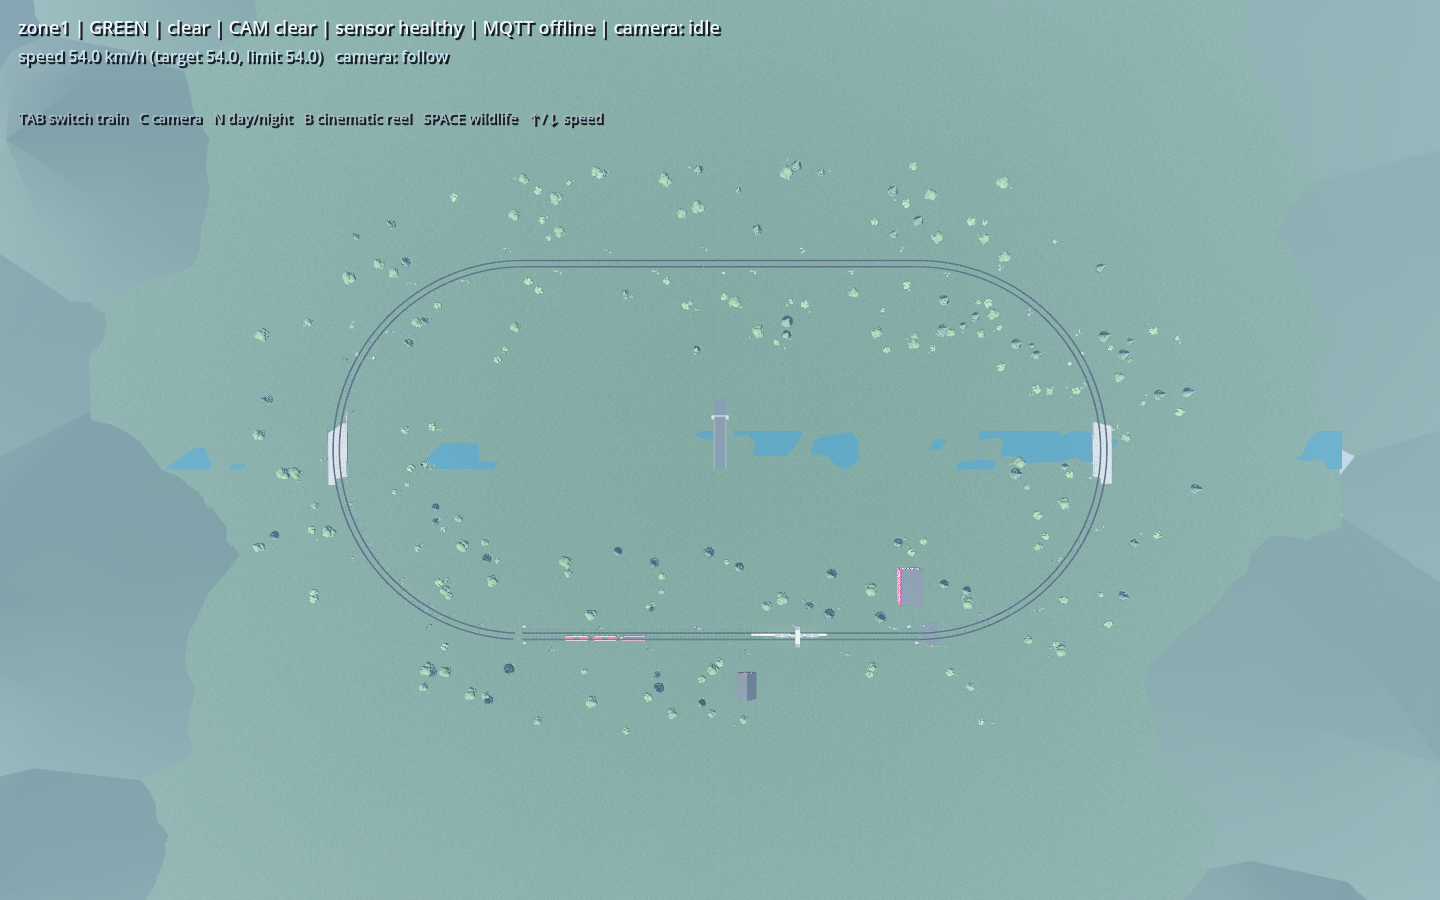
\includegraphics[width=16.8cm]{double_track_overview.png}
\caption{Top-down overview of the shared stadium footprint: UP and DOWN
tracks, the island station platform, carved river with a road and a railway
bridge, tree line, and the two-train fleet (HUD shows the active zone,
signal aspect, CAM state, sensor health, speed and camera mode). Captured
from \texttt{capture\_double\_track.gd} under headless software rendering;
the HUD \texttt{MQTT offline} flag is expected in capture mode where the
broker is intentionally not connected.}
\label{fig:overview}
\end{figure}

\begin{itemize}
  \item \textbf{Stadium double-track geometry:} UP and DOWN loops share a
        250\,m straight-sided stadium footprint --- centre lines
        \texttt{z = $\pm$120\,m}, straights \texttt{x = $-125..125$\,m},
        east/west curves of radius 120\,m. Closed lengths are UP
        1253.9822\,m and DOWN 1228.8495\,m, with block lengths 250.796\,m
        and 245.77\,m respectively (verified in \texttt{test\_stadium\_track}
        and \texttt{test\_geometry.test.js}).
  \item \textbf{Opposite running:} T1 runs clockwise on UP; T3 runs
        anticlockwise on DOWN with DOWN chainage converted
        (operational vs physical) and the opposite face---based on where
        the train is --- hidden from wildlife spawning logic
        (\texttt{test\_opposite\_running}).
  \item \textbf{Carved river and bridges:} a procedural river channel
        through the stadium with a road bridge and two widened railway
        bridge decks positioned at the track crossings; piers clear both
        rails and no tree is planted within 5\,m of either centre line
        (\texttt{test\_river\_bridges}, \texttt{test\_corridor\_flatten}).
  \item \textbf{Catenary and signals:} catenary wire runs above both
        lines; block signal masts display per-block aspects from the
        backend (\texttt{test\_catenary\_double},
        \texttt{test\_signal\_masts}).
\end{itemize}

\section{Island station and interlocked crossovers}

The island platform sits inside backend block UP-B2/DOWN-B2, built from
identical 9.6$\times$1.8$\times$2.2\,m modules with a canopy, benches and
bins (\texttt{test\_station\_island}); the platform spans chainage 150--198\,m
on the south straight.

\begin{figure}[H]
\centering
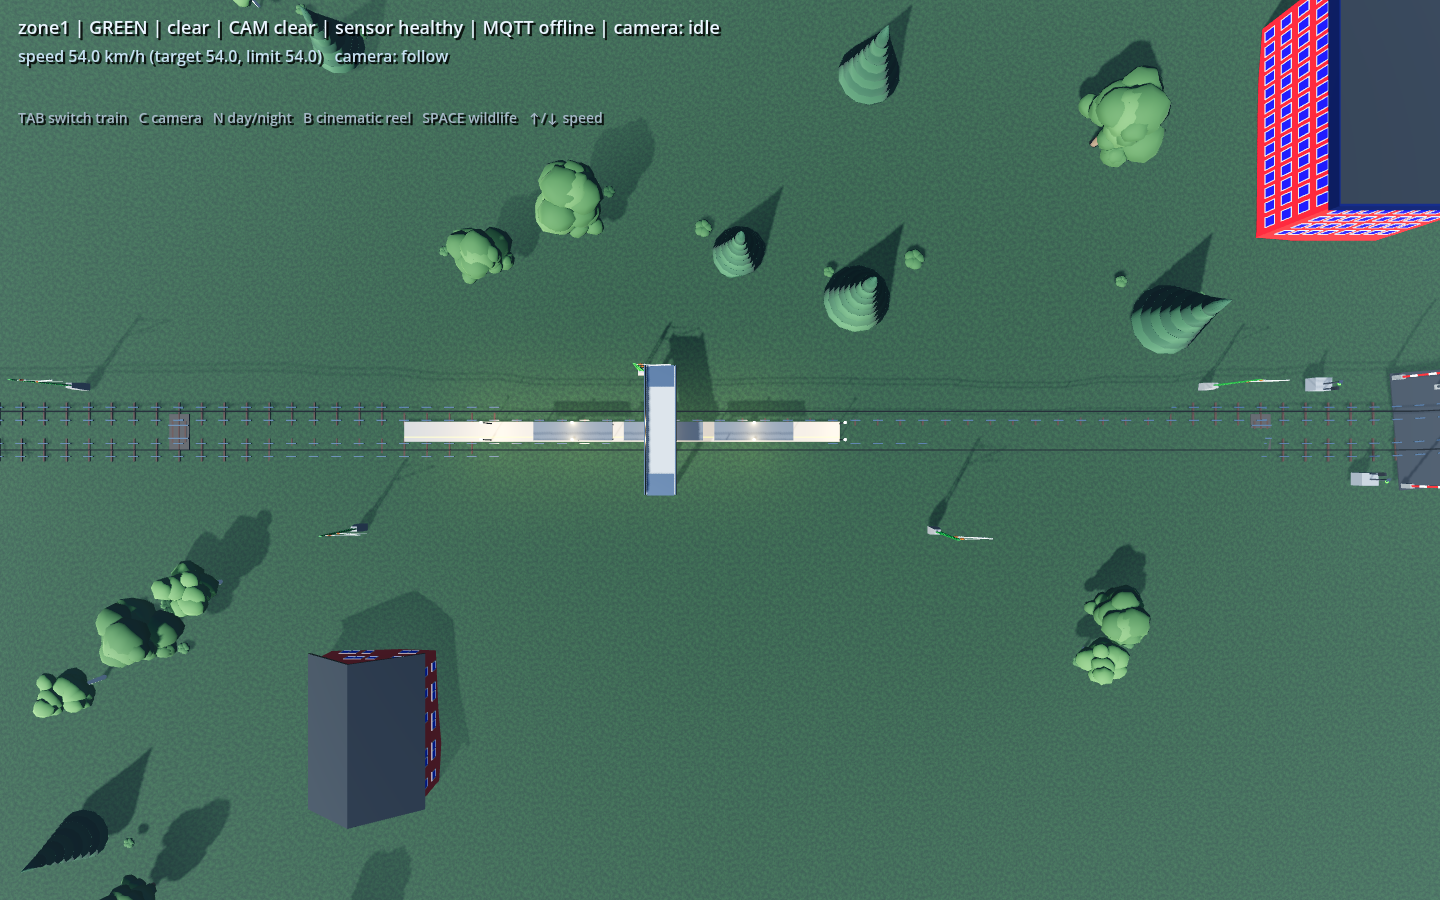
\includegraphics[width=16.8cm]{platform_after_topdown.png}
\caption{Island station from above: mainly-top view showing platform
modules, canopy/station building, both platforms and the two tracks.
Captured from \texttt{capture\_station.gd}.}
\label{fig:platform-topdown}
\end{figure}

\begin{figure}[H]
\centering
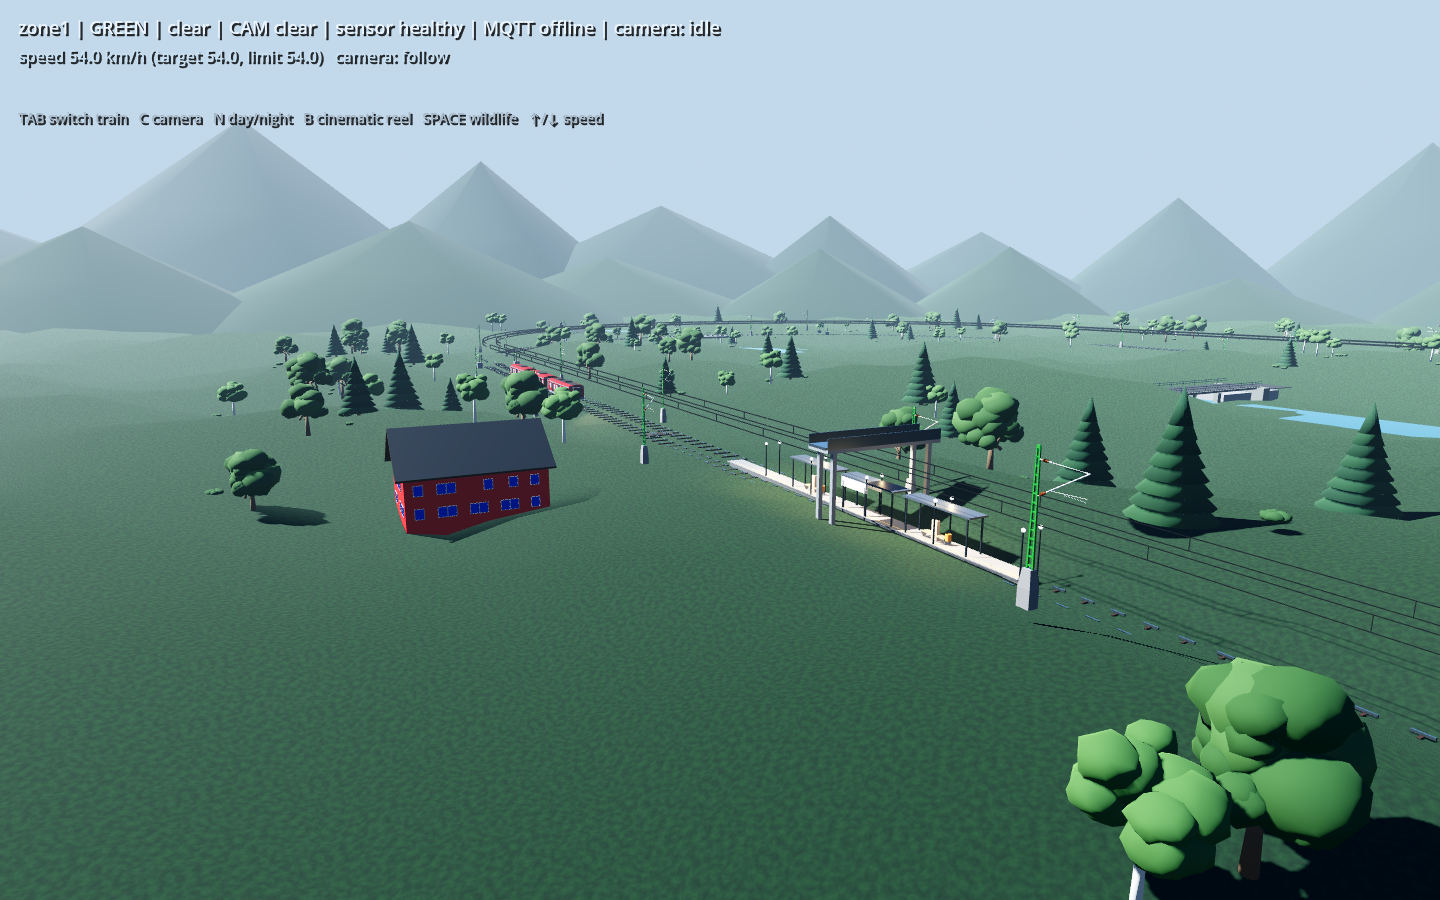
\includegraphics[width=16.8cm]{platform_after_oblique.png}
\caption{Island station at an oblique angle: platform modules and canopy
silhouette against \\ the parallel tracks and stadium corridor in the
background. Captured from \texttt{capture\_station.gd}.}
\label{fig:platform-oblique}
\end{figure}

Two station crossovers interlock the loops: \textbf{Crossover A} at UP
chainage 120\,m and \textbf{Crossover B} at UP chainage 240\,m, both ending
on both centre lines with visible switch blades
(\texttt{test\_station\_crossovers}). Routes are only granted through the
backend interlock (\texttt{routes.requestRoute}) and occupancy, hazard and
restrictive-zone checks are unchanged in every route type.

\section{Wrong-line run across the station}

An operator can request an interlocked wrong-line run: the requesting train
crosses from UP to DOWN at A, runs against traffic on the DOWN line, and
crosses back at B, while the opposing train is automatically held at a
point outside B inside braking distance.

\begin{figure}[H]
\centering
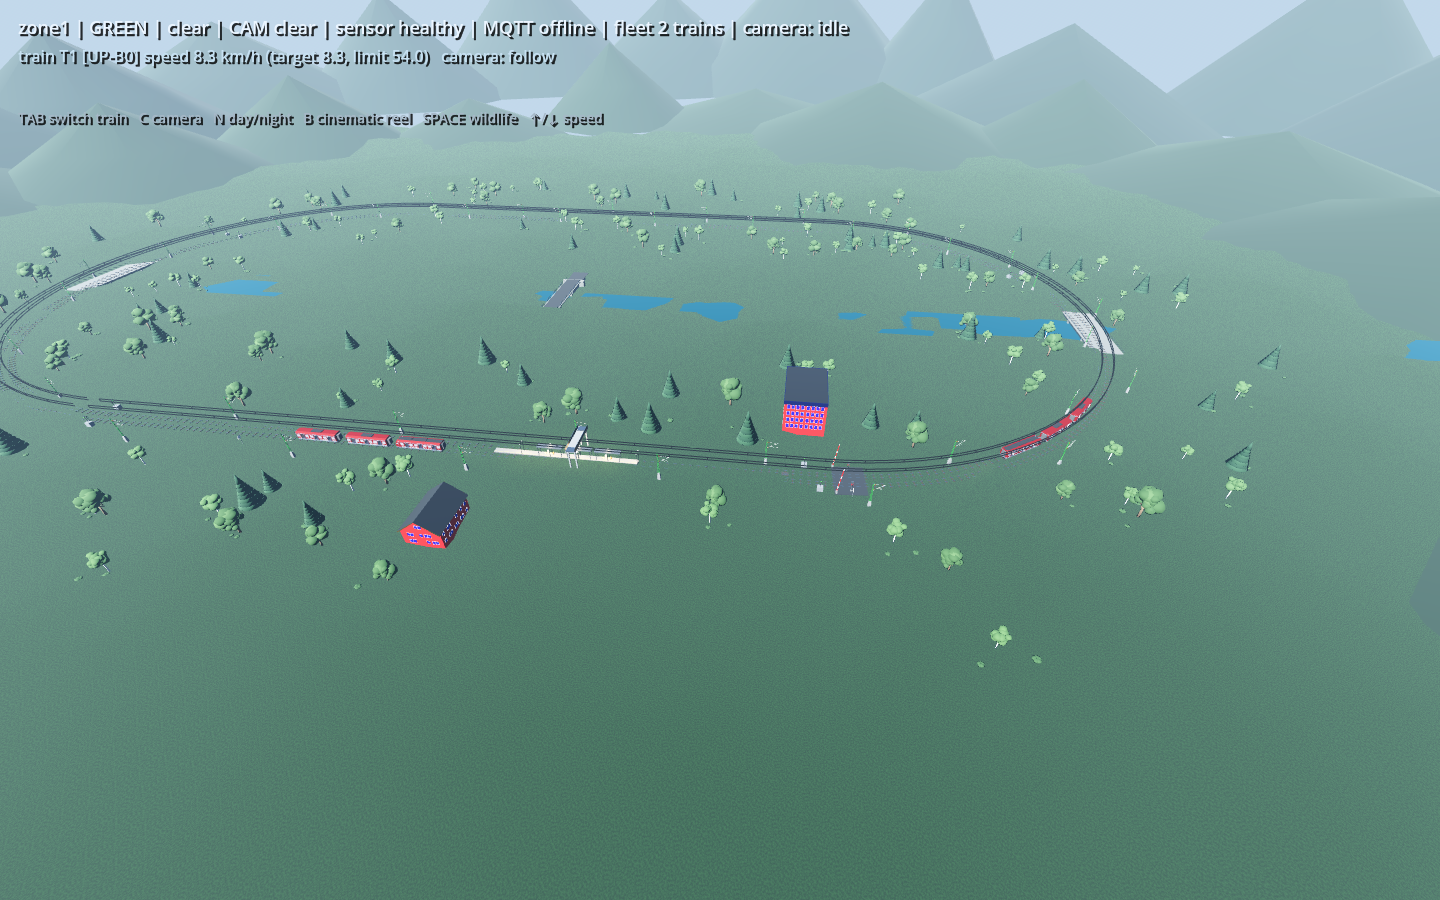
\includegraphics[width=16.2cm]{wrong_line_before.png}
\caption{Wrong-line run at UP phase APPROACH: T3 still on DOWN, T1
approaching crossover A before any visible motion; note HUD hold progress.
Captured from \texttt{capture\_crossover.gd}.}
\label{fig:wronglinebefore}
\end{figure}

\begin{figure}[H]
\centering
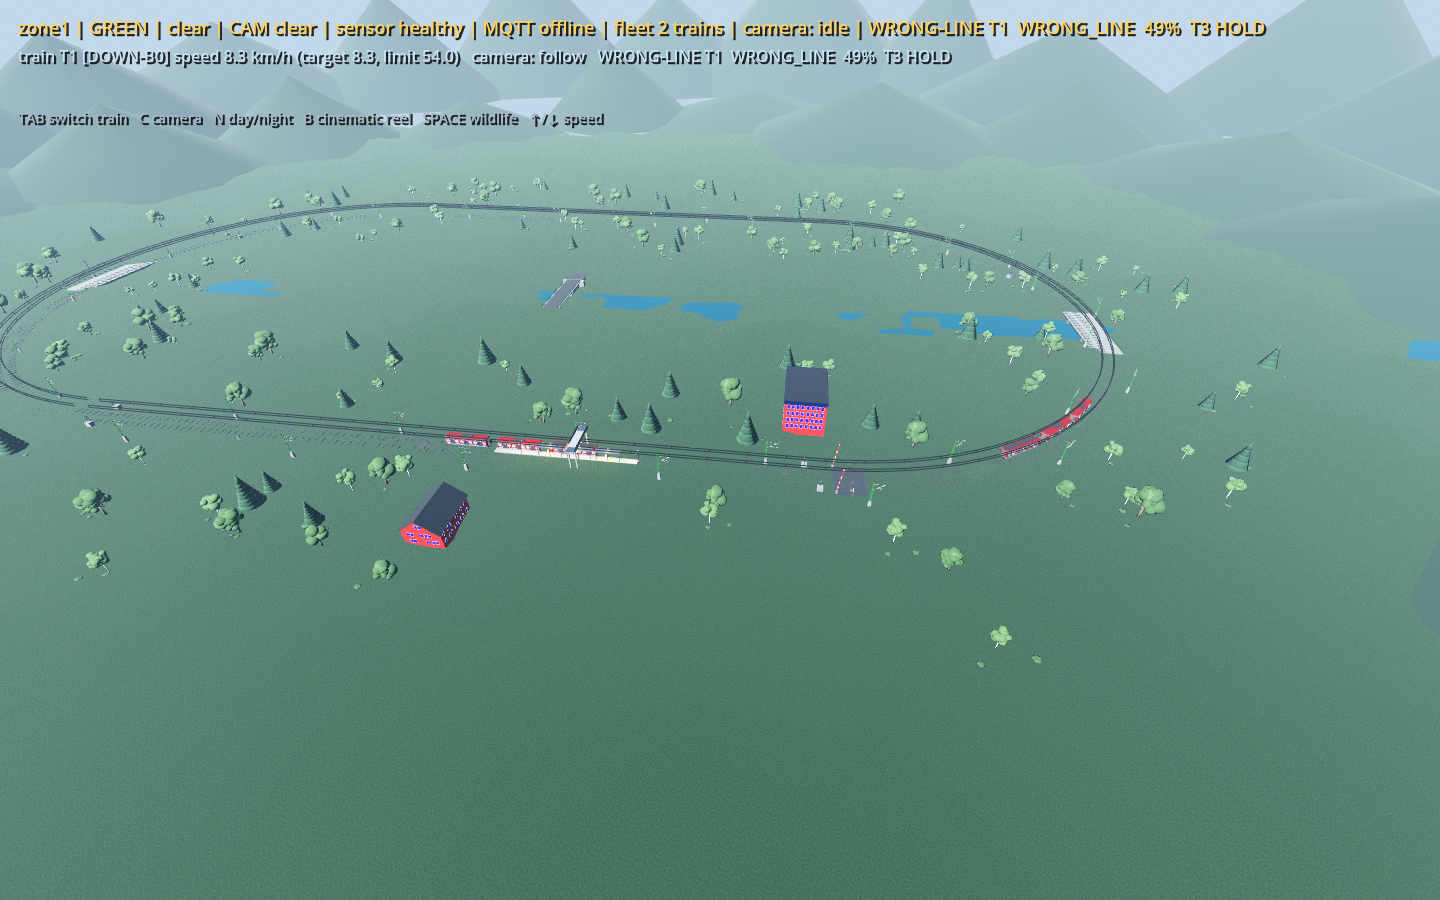
\includegraphics[width=16.2cm]{wrong_line_midway.png}
\caption{Wrong-line run at phase CROSS\_ENTRY/WRONG\_LINE: T1 blended onto
DOWN at A -- visible train between the switch points with switch blades in
motion. Captured from \texttt{capture\_crossover.gd}.}
\label{fig:wronglinemidway}
\end{figure}

\begin{figure}[H]
\centering
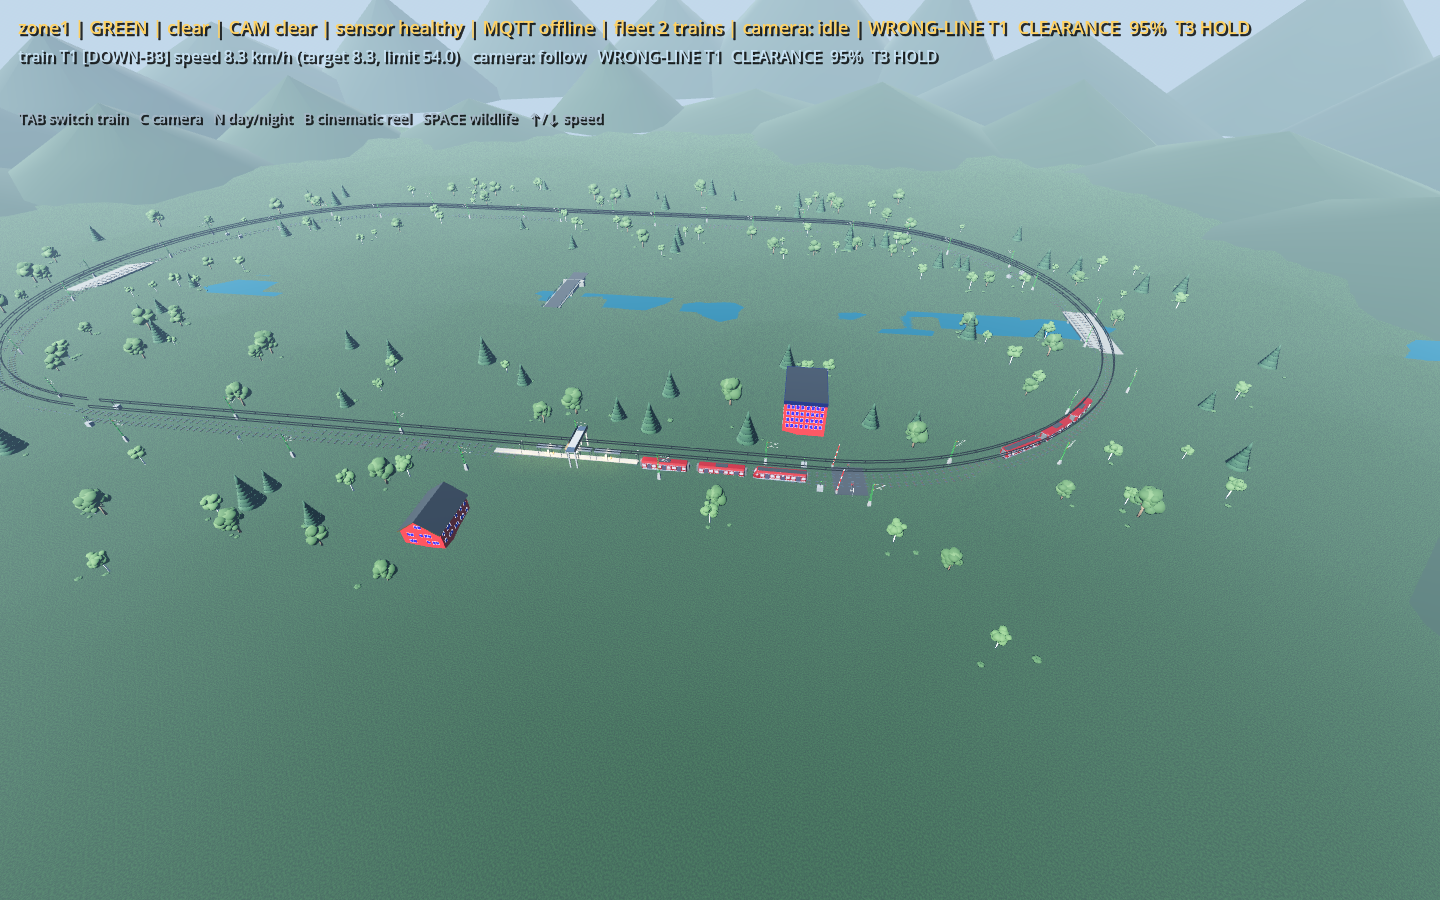
\includegraphics[width=16.2cm]{wrong_line_after.png}
\caption{Wrong-line run completion (phase CROSS\_EXIT/CLEARANCE): T1 back
on UP past B, T3 released from hold and both trains back under normal
authority. Captured from \texttt{capture\_crossover.gd}.}
\label{fig:wronglineafter}
\end{figure}

The visible crossover blend is backend-driven --- trains smoothly change
track without a snap; \texttt{test\_crossover\_visual} asserts smooth
movement across the join with no apply-state jump.

\section{Chance-based meets}

A seeded PRNG scheduled the meets the operator can trigger or let happen
naturally. A trigger window holds one of the two trains at the station
with \texttt{commandedSpeedKmh=0} at the backend so the meet only happens
when the other train is near; completion uses a proper interlocked
crossover route.

\begin{figure}[H]
\centering
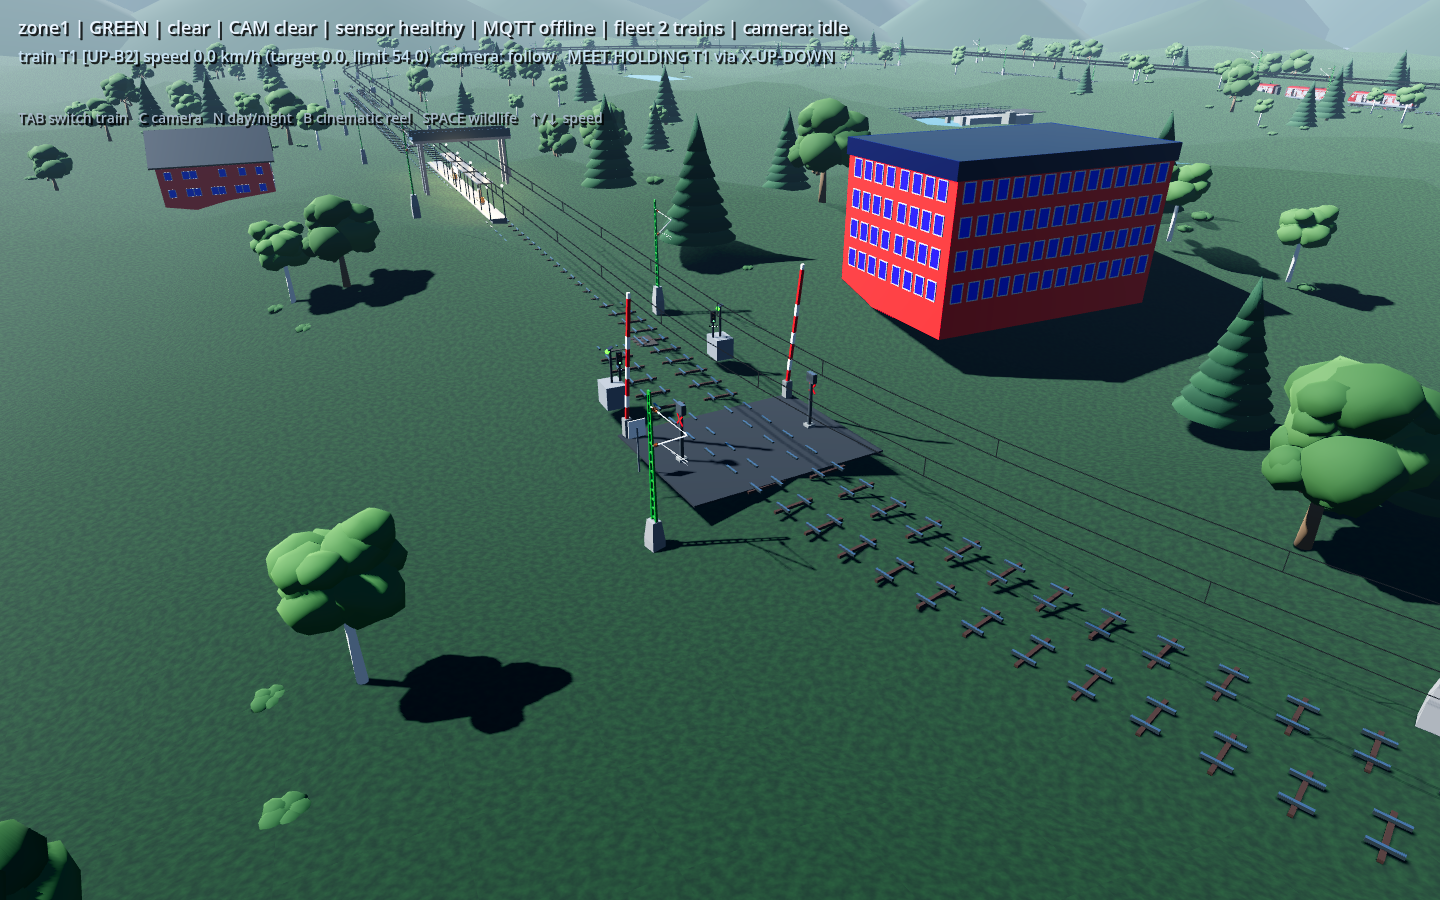
\includegraphics[width=16.8cm]{meet_randomized.png}
\caption{Live meet execution with seed 4242: both trains near the island
platform, one held, with the meet HUD showing phase, holder, chosen route
and countdown. Captured from \texttt{capture\_meet.gd}.}
\label{fig:meet}
\end{figure}

\section{The LTS asset fleet}

The twin replaces procedural stubs with real \textbf{Libre-TrainSim}
(LTS) exports: the train consist GLBs (cab car and
coaches), the island station modules, plus deer and elephant animals with
articulated limbs (verified by \texttt{test\_real\_assets}, which checks
the GLBs have landed in the scene graph and are placed on the correct
track). \texttt{tools/export\_lts\_assets.py} / \texttt{.sh} convert the
LTS Blender source files; \texttt{godot/assets.manifest.json} records
asset provenance and paths.

\begin{figure}[H]
\centering
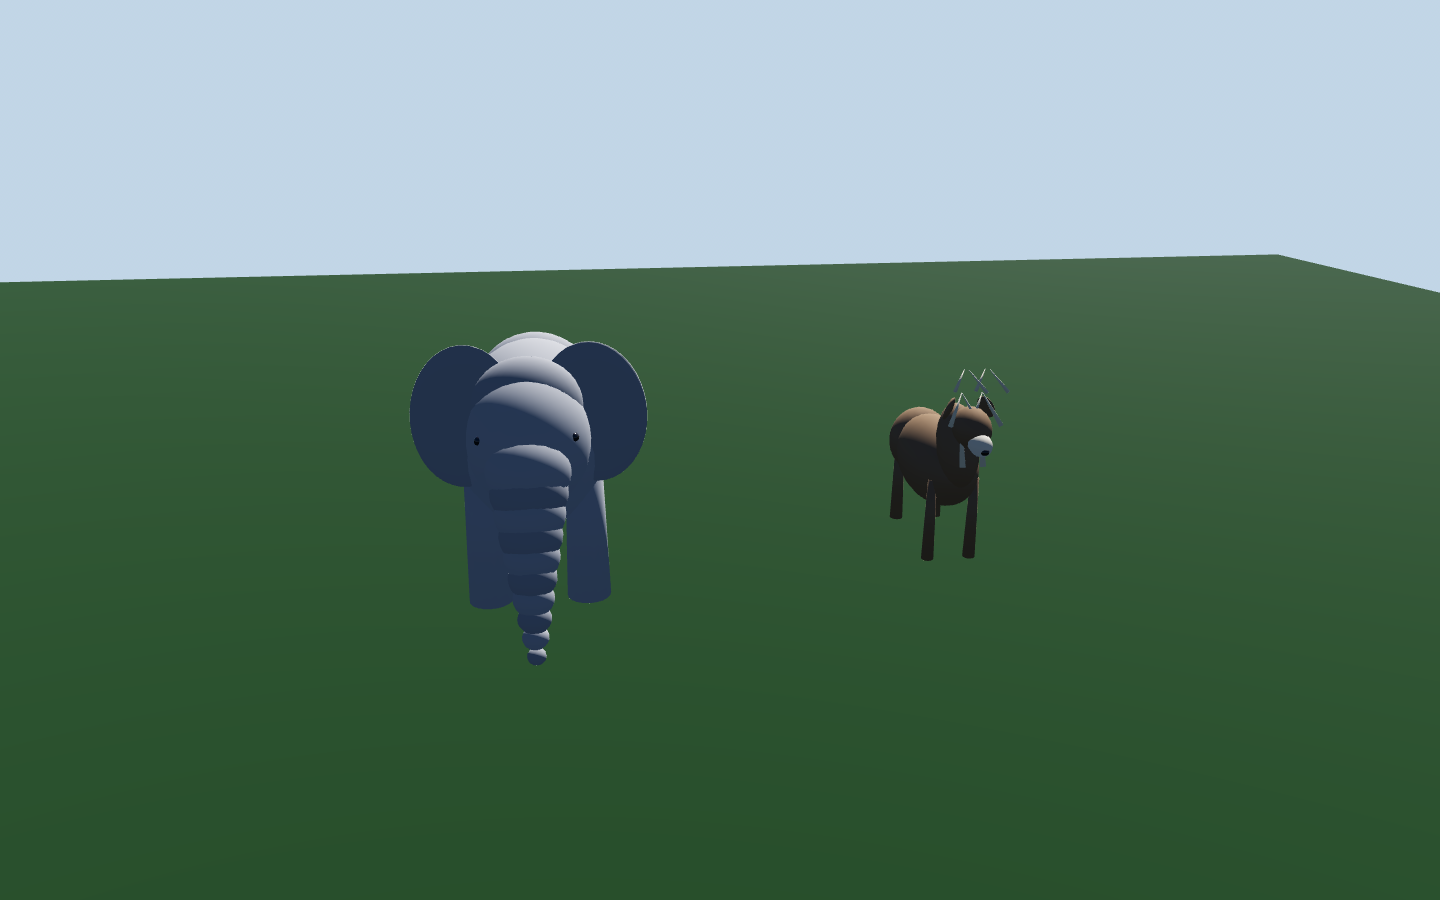
\includegraphics[width=16.2cm]{animals_scene.png}
\caption{Wokwi-style animal-assets sanity render: deer and elephant GLBs
with articulated limbs posed near the track, plus the sensor hut and
barrier kit. Captured from \texttt{capture\_animals.gd}.}
\label{fig:animals}
\end{figure}

Figure~\ref{fig:cameraconfirm} (Chapter~\ref{cha:dashboards}) shows the
same fleet in the live safety chain confirmed elephant ahead at 0.95/
confidence with a STOP already applied by the twin.

\section{Operator and observer surfaces of the twin}

\begin{itemize}
  \item \textbf{Keyboard:} \texttt{SPACE} toggles a zone-1 wildlife event,
        \texttt{F} toggles the sensor fault, \texttt{R} resets (only with
        all clear), \texttt{Up/Down} adjust local target speed
        (8\,km/h steps), \texttt{2} toggles zone-2 wildlife,
        \texttt{C} cycles camera modes (four modes, incl.\ orbit and
        onboard), \texttt{N} day/night.
  \item \textbf{HUD:} a debug bar continuously reports zone state, signal,
        CAM/HUT evidence path, sensor health, backend connection,
        camera status and speed; fleet-level HUD adds per-train lines, and
        the wrong-line HUD shows phase and percentage progress plus the
        opposing train hold state (\texttt{test\_wrong\_line\_hud}).
  \item \textbf{Camera director:} choose mode with \texttt{C}; capture
        scripts reuse the same director for deterministic angles used in
        the gates and in this report.
\end{itemize}

\section{Twin subsystem modules}

\begin{longtable}{>{\raggedright}p{4.0cm} >{\raggedright\arraybackslash}p{11.6cm}}
\caption{Key \texttt{godot/src} modules}\label{tab:twinmodules}\\
\toprule
\textbf{Module} & \textbf{Responsibility} \\
\midrule
\endfirsthead
\caption[]{(continued)}\\
\toprule
\textbf{Module} & \textbf{Responsibility} \\
\midrule
\endhead
\texttt{mqtt\_bridge.gd} & MQTT inbound/outbound with exponential backoff on broker failure \\
\texttt{train\_reconciler.gd} / \texttt{fleet\_controller.gd} & Apply authoritative backend state to the twin fleet (speeds, signals, routes) \\
\texttt{track\_registry.gd} / \texttt{ltstrack.gd} / \texttt{track\_builder.gd} & Stadium track geometry, chainage conversion, mesh building \\
\texttt{level\_crossing.gd} & Two-track level crossing: alarms, pivoting booms, light logic \\
\texttt{wildlife\_director.gd} / \texttt{wildlife\_spawner.gd} & Deterministic seeded wildlife appearances at correct chainage and distance \\
\texttt{wildlife\_safety.gd} / \texttt{animal\_safety\_system.gd} & Local fail-safe layers with backend precedence logic \\
\texttt{onboard\_braking.gd} / \texttt{detection\_band.gd} & Quadratic stopping-distance and safe-speed inversion \\
\texttt{animal\_detector.gd} / \texttt{camera\_confirmation.gd} & Simulated forward camera (cone, occlusion) and evidence upload \\
\texttt{trackside\_sensor\_hut.gd} / \texttt{wildlife\_sensor\_network.gd} & Distributed hut observations \\
\texttt{block\_signal\_mast.gd} / \texttt{safety\_signals.gd} & Visual per-block aspects \\
\texttt{camera\_director.gd} / \texttt{twin\_hud.gd} & Cameras and the HUD overlaid in captures \\
\bottomrule
\end{longtable}

% ============ CHAPTER 7 — DASHBOARDS ============
\chapter{Dashboards}\label{cha:dashboards}

\section{The web operations dashboard}

The dashboard (\texttt{web/src/App.tsx}, React 18 + TypeScript, served on
port 5173) is the operator- and admin-facing surface. It talks to the
backend over two channels: authenticated REST for every control, and the
backend event stream over WebSocket for live truth. It performs no
transformation of state: what it shows is what the backend published.

\subsection{Login and role awareness}

\begin{itemize}
  \item Login screen posts \texttt{username}/\texttt{password} to
        \texttt{/api/login} (bcrypt-verified) and holds the returned JWT
        in memory for every subsequent REST call.
  \item Three seed roles: \textbf{viewer} observes, \textbf{operator} may
        issue controls, \textbf{admin} additionally inspects the audit
        trail; the UI derives affordances from the role map returned with
        the token, and --- critically --- the backend re-checks every
        request independently, so the UI cannot grant what the token
        forbids.
  \item The top bar shows the authenticated user, the MQTT connection
        state pill (live \texttt{state.mqttConnected}) and a clock.
\end{itemize}

\subsection{Panels and data flow}

Panels\footnote{Panel names are the literal \texttt{<h3>} strings in
\texttt{App.tsx}, observed in the source at the time of writing.} in
rendered order:

\begin{longtable}{>{\raggedright}p{4.6cm} >{\raggedright\arraybackslash}p{5.6cm} >{\raggedright\arraybackslash}p{4.7cm}}
\caption{Dashboard panels}\label{tab:dashpanels}\\
\toprule
\textbf{Panel} & \textbf{Content} & \textbf{Backing data} \\
\midrule
\endfirsthead
\caption[]{(continued)}\\
\toprule
\textbf{Panel} & \textbf{Content} & \textbf{Backing data} \\
\midrule
\endhead
Hero scenario express actions & One-click \texttt{Inject wildlife event} and \texttt{Simulate sensor fault}; an animated scene card with train, live signal head and \texttt{WILDLIFE ZONE} marker & \texttt{POST /api/control} envelope \\
Fleet grid (train cards) & One card per train (T1/T3): current vs target speed, occupied block, UP/DOWN line pill, \texttt{CLOCKWISE}/\texttt{ANTICLOCKWISE} direction; select a card to drive its speed control & retained \texttt{railway/state} snapshot via WS \\
Fleet Speed \& Hazard Controls & Per-train target speed with slider and \texttt{RESET}/\texttt{Clear wildlife}/\texttt{Restore sensor} actions & \texttt{POST /api/speed \{trainId\}}; control envelopes \\
Station Hold Scheduler (meet card) & Meet seed, phase, holder train, chosen route and countdown to next window & \texttt{POST /api/meet}, snapshot \texttt{meets} \\
Wrong-Line Run panel & Operator-requested wrong-line: eligibility display, start and cancel, with hold and clearance states streaming in & \texttt{POST /api/wrong-line}, snapshot \texttt{wrongLine} \\
Sensor $\rightarrow$ Camera $\rightarrow$ Stop (wildlife card) & Stage (\texttt{NONE}/\texttt{SUSPECTED}/\texttt{CONFIRMED}), evidence sources (HUT/CAM/ESP32 tags), confidence, species, camera health (\texttt{ONLINE}/\texttt{DEGRADED}), ML status (\texttt{STUB}/\texttt{LOADED}), near-warning (30\,km/h) & hazard snapshot + \texttt{/api/camera/health} \\
Authoritative Block Signalling \& Occupancy & Block-by-block diagram with per-block aspects (RED/YELLOW/GREEN), occupancy side, CAM/HUT evidence badges on hazard blocks & snapshot blocks + retained \texttt{railway/signal/\{block\}} \\
Audit \& Operations Log & Live event stream (type, message, time, source, severity) --- admin-invisible events are still validated backend-side; audit rows themselves are admin/backend-inspectable & WS event stream \\
Wokwi ESP32 (communicator kernel) & ESP32 device health, zone, telemetry freshness --- the state of the edge node at a glance & \texttt{railway/telemetry/esp32} relay via snapshot \\
\bottomrule
\end{longtable}

\subsection{Evidence badges on the block diagram}

During a hazard, the block diagram tags the involved block with its
evidence sources --- \texttt{CAM} (onboard simulated camera),
\texttt{HUT} (trackside sensor network) or \texttt{ESP32} (edge device) ---
so an operator can immediately see which surfaces agreed, matching the
backend's dual-evidence fusion model (Section~\ref{sec:features-wildlife}).

\section{The twin-side HUD}

The 3D twin carries its own HUD so the information survives even when the
web dashboard is closed:

\begin{itemize}
  \item \textbf{Debug/state bar} (top of every render): zone state,
        signal aspect, \texttt{WILDLIFE}/\texttt{CAM}/\texttt{clear}
        evidence and confidence, sensor health, MQTT connection flag,
        camera status and per-train speed (target and limit) shown in
        \texttt{km/h}.
  \item \textbf{Fleet HUD} (\texttt{test\_fleet\_hud}): per-train lines ---
        speed, block, line, direction --- for both trains simultaneously.
  \item \textbf{Meet HUD} (\texttt{test\_meet\_hud}): phase, holder,
        route and the countdown to the next meet window; tolerated as
        absent when the backend snapshot predates meets.
  \item \textbf{Wrong-line HUD} (\texttt{test\_wrong\_line\_hud}):
        \texttt{WRONG-LINE T1 <phase> <pct>\% T3 HOLD} rendered from the
        backend route state.
  \item \textbf{Camera confirmation HUD}: \texttt{CAM detect}/
        \texttt{CAM clear} plus the confirmed species and confidence ---
        shown in Figure~\ref{fig:cameraconfirm}.
\end{itemize}

\begin{figure}[H]
\centering
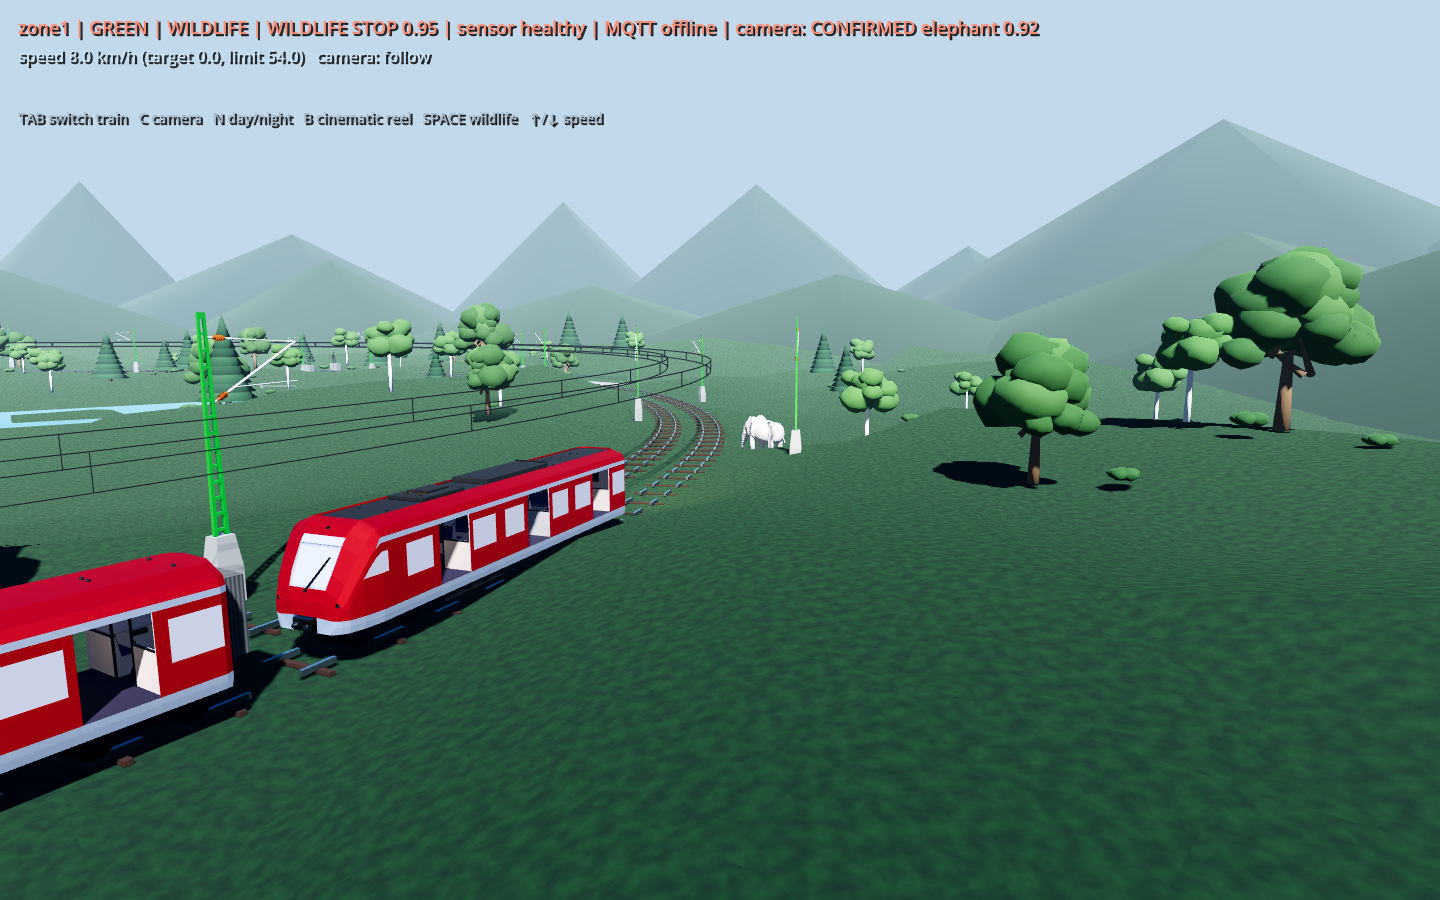
\includegraphics[width=16.8cm]{camera_confirm.png}
\caption{Twin HUD during a confirmed wildlife stop: top bar reads
\texttt{WILDLIFE | WILDLIFE STOP 0.95 | camera: CONFIRMED elephant 0.92}
--- target speed 0, limit 54, camera tracking from behind
the red LTS train. The elephant detection ahead is the simulated render
that produced the confirmed evidence. Captured from
\texttt{capture\_camera\_confirm.gd}.}
\label{fig:cameraconfirm}
\end{figure}

\section{Diagnostics surfaces}

\begin{itemize}
  \item \textbf{Backend health:} \texttt{GET /api/health} returns
        \texttt{\{"ok":true,"mqttConnected":true\}} --- the single command
        every operator first runs (\texttt{dev-up.sh} waits on it for
        up to 60\,s).
  \item \textbf{Audit inspection:} admin surfaces audit rows (actor, role,
        zone, action, result, timestamp) from the SQLite audit table via
        the authenticated endpoint; every control attempt appears here
        regardless of acceptance.
  \item \textbf{Broker observability:} Mosquitto logs all connections;
        ACL denials are visible in \texttt{docker compose logs mqtt} ---
        the fastest way to diagnose a mis-scoped client.
  \item \textbf{Wokwi panel:} the dashboard's ESP32 card exposes the last
        telemetry timestamps, so the edge node's freshness is visible
        without reading serial.
\end{itemize}

\section{Two dashboards, one truth}

A deliberate design property: the web dashboard and the twin HUD are two
renderings of the same backend-published state, and the backend is the
sole publisher. The twin never silently widens permissions, and the
dashboard never invents state: if the twin disagrees with a command, the
discrepancy appears in the HUD's own limit versus the backend's target
(e.g.\ the local limit only \emph{tightens} a target, never loosens it).

% ============ CHAPTER 8 — FEATURES AND FUNCTIONS IMPLEMENTED ============
\chapter{Features and Functions Implemented}\label{cha:features}

This chapter is the master inventory: every shipped capability, where it
lives, and the test evidence that gates it. Evidence rows cite
\texttt{docs/porting/acceptance.md} --- the formal acceptance
record) and named suites under \texttt{backend/test/},
\texttt{godot/tests/}, \texttt{esp32/test/} and \texttt{ml/tests/}.

\section{Backend: authority, safety and security}

\begin{longtable}{>{\raggedright}p{5.0cm} >{\raggedright\arraybackslash}p{5.6cm} >{\raggedright\arraybackslash}p{4.6cm}}
\caption{Backend features}\label{tab:backend-features}\\
\toprule
\textbf{Feature} & \textbf{Where} & \textbf{Evidence} \\
\midrule
\endfirsthead
\caption[]{(continued)}\\
\toprule
\textbf{Feature} & \textbf{Where} & \textbf{Evidence} \\
\midrule
\endhead
Login with bcrypt + JWT; RBAC viewer/operator/admin & \texttt{auth.js}, \texttt{rbac.js} & \texttt{auth.test.js}, \texttt{rbac.test.js} \\
Command-envelope validation: schema + $\pm$5\,min freshness & \texttt{validate.js} & \texttt{validate.test.js} \\
Anti-replay via persistent SQLite registry & \texttt{command\_tracker.js}, \texttt{replay.js} & \texttt{replay.test.js} \\
Audit row for every accepted/rejected/forbidden attempt & \texttt{audit.js} & every control test asserts audit rows \\
Two-zone then two-train fleet state machine & \texttt{state.js}, \texttt{simulation.js} & \texttt{state.test.js}, \texttt{simulation.test.js} \\
Ten-block per-block aspects with retained signals & \texttt{signalling.js}, \texttt{bus.js} & \texttt{signalling.test.js}, \texttt{bus.test.js} \\
Occupancy safety: never overtake onto a RED block; own-overlap allowance & \texttt{simulation.js} & \texttt{simulation.test.js} (boundary + overlap case \texttt{f55f872}) \\
Station-crossover interlock + route lifecycle & \texttt{routes.js} & \texttt{routes.test.js}; 409 on occupied destination; audited \texttt{route:set} \\
Chance-based meet scheduler from seeded PRNG & \texttt{meets.js}, \texttt{rng.js} & \texttt{meets.test.js}, \texttt{rng.test.js} \\
Wrong-line run with phases and opposing hold & \texttt{wrong\_line.js} & \texttt{wrong\_line.test.js}, \texttt{wrong\_line\_api.test.js} \\
Fixed-timestep 2\,Hz authority loop on MQTT connect & \texttt{loop.js}, \texttt{server.js} & \texttt{loop.test.js} \\
\texttt{COMM\_LOST} fail-safe and retained-state reconciling & \texttt{mqtt.js}, \texttt{events.js} & \texttt{broker\_acl/e2e} suites \\
Trackside observation $\rightarrow$ block RED + approach YELLOW; opposite line unaffected & \texttt{wildlife\_commands.js} & \texttt{wildlife\_observation.test.js} \\
Camera ingest (token, freshness, dup id, size/rate limits, evidence cap, block/line match) & \texttt{ingest.js}, \texttt{ml.js} & \texttt{camera.test.js} (9/9 incl.\ 413, 429, 503-functional) \\
Two-frame confirmation policy; near vs confirmed; clear never downgrades confirmed & \texttt{wildlife\_commands.js} & \texttt{near\_animal.test.js} (9/9) \\
ESP32 command forwarding + zone gating + \texttt{RESET} relay & \texttt{routes/wildlife.js} & \texttt{wildlife\_observation.test.js}, firmware native suite \\
Legacy anonymous \texttt{POST /api/event} deleted (404) & \texttt{app.js} & \texttt{control\_routes.test.js} \\
\bottomrule
\end{longtable}

\section{Wildlife protection chain}\label{sec:features-wildlife}

The headline safety feature is the fully assembled chain:

\begin{enumerate}
  \item \textbf{NONE (normal):} all sensors healthy, train at target.
  \item \textbf{SUSPECTED:} a trackside hut observation (or a single camera
        frame, or an ESP32 pull) makes the involved block YELLOW and caps
        the approaching train at \textbf{30\,km/h} with a
        \texttt{WILDLIFE\_NEAR} warning delivered to ESP32.
  \item \textbf{CONFIRMED:} a second camera frame --- the two-frame
        evidence policy, \texttt{camera.test.js} is authoritative ---
        confirms (species + confidence, e.g.\ elephant 0.92). Backend
        sets block \textbf{RED}, train target \textbf{0\,km/h},
        \texttt{STOP}/\texttt{WILDLIFE\_DETECTED} to the edge node, twin
        shows STOP with barriers down.
  \item \textbf{Clearing:} the sensor clear never downgrades a confirmed
        block; the backend latches \texttt{RECOVERY\_REQUIRED} (RED until
        reset).
  \item \textbf{RESET:} an authorized operator/admin sends RESET with no
        active hazard or sensor fault; the backend returns the zone to
        \texttt{NORMAL}, sends \texttt{RESET} to ESP32, and keeps the
        train at 0 until an explicit \texttt{/api/speed} re-arms it.
\end{enumerate}

Local backup layer: the twin's own detector fires zero-latency braking
(\texttt{set\_local\_wildlife\_limit(0)}) even with MQTT offline, and the
ESP32's local inputs produce restrictive outputs regardless of network
state --- three independent protectors on the same event.

\subsection{Onboard simulated vision}

\begin{itemize}
  \item Forward cone vision: horizontal $\pm$25$^\circ$, vertical
        $\pm$10$^\circ$, 180--200\,m range (per
        \texttt{test\_onboard\_detector}).
  \item Confidence scoring (deer 0.9, elephant 1.1 modifiers) and
        \textbf{analytic occlusion} against the terrain hill, tree trunks
        and bridge decks.
  \item A camera aligned with the carriage forward tangent
        (dot $> 0.98$ checked across curves,
        \texttt{test\_onboard\_camera}), uploading frames with
        \texttt{X-Captured-At} (UTC, Z-suffixed) and
        \texttt{X-Block} naming the hazard block ahead (not the train's
        current block), filtered inside 200\,m by operational distance.
  \item Pure quadratic stopping-distance model
        $d_{\text{stop}}(v) = v\,t_r + \tfrac{v^2}{2a_{\text{brake}}} + d_{\text{margin}}$
        (56\,m at 36\,km/h) with the safe-speed limit inverted from it;
        \texttt{test\_onboard\_braking} pins the numbers.
\end{itemize}

\section{Twin features}

Summarised from Chapter~\ref{cha:twin}: stadium double-track world with
verified geometry, island station with two interlocked visible crossovers,
two-track wildlife level crossing with boom barriers and alarm, river with
road + railway bridges, catenary, block signal masts, LTS-derived
train/station/animal GLB fleet, deterministic wildlife director,
sensor-hut network (10 huts, 75\,m overlapping radius) with status lamps,
camera director, day/night, multi-cam HUD, wrong-line visual blend
without snapping, and meet-hold rendering.

\section{ESP32 and edge features}

Summarised from Chapter~\ref{cha:hardware}: authenticated broker identity,
non-blocking reconnect and telemetry, restrictive-first outputs from boot,
distinguishing behavior between local wildlife, local fault, comm loss,
backend stop and near-warning states, SNTP-gated clock truth, edge-triggered
\texttt{WILDLIFE\_NEAR}/\texttt{WILDLIFE\_DETECTED} rendering with buzzer
pulses, and zone-scoped command validation --- the whole decision core
covered by 16 native Unity cases and live Wokwi scenarios.

\section{ML service features}

\begin{itemize}
  \item JPEG-frame detection endpoint returning animal classes with
        confidence and bbox; health endpoint exposing
        \texttt{modelLoaded}/stub state and readiness.
  \item Real-weights path with torchvision
        \texttt{ssdlite320\_mobilenet\_v3\_large} filtered to COCO animal
        labels; weights cached under \texttt{ml/.cache}.
  \item \texttt{ML\_STUB=1} deterministic elephant detection
        (\texttt{modelLoaded: true}, 0.92) so integration segments run
        without torch downloads --- most verification runs in this mode;
        the real-model path was smoke-skipped for lack of cached weights
        and covered instead by input-validation tests (image decoded
        before model load; invalid images rejected even with
        \texttt{ML\_STUB=1}).
  \item Edge coverage: oversized payload 413, detector crash 503, and
        non-stub image rejection tests in \texttt{ml/tests/}.
\end{itemize}

\section{Dashboard features}

Summarised from Chapter~\ref{cha:dashboards}: authenticated login with
role-aware affordances, live fleet grid with per-train direction/speed,
station hold scheduler card, wrong-line operator panel with eligibility
and cancel, block diagram with aspects and CAM/HUT/ESP32 evidence badges,
wildlife stage/evidence panel with camera health and ML status, seed-driven
meet card, event stream, ESP32 health card and one-scenario hero actions.

\section{Safety behaviour and edge cases (cross-cutting)}\label{sec:features-safety}

The edge cases that the suites actually pin:

\begin{itemize}
  \item \textbf{Duplicate suppression:} duplicate event IDs (camera ingest
        and ESP32 observations) are ignored without re-arming alarms.
  \item \textbf{Rate and size guards:} camera ingest rejects $>$5\,fps
        input with 429 and oversize bodies with 413; evidence files are
        capped and pruned to 50.
  \item \textbf{Range filtering:} camera confirmation ignores hazards
        behind the train or beyond 200\,m operational distance.
  \item \textbf{Zone gates:} an ESP32 command outside \texttt{ESP32\_ZONE}
        is never forwarded; the device validates the zone again on receipt.
  \item \textbf{Replay and stale data:} timestamp $\pm$5\,min window;
        dedupe by request id; no queued old telemetry/commands on device
        reconnect.
  \item \textbf{Local dominance:} local wildlife/fault inputs override
        backend commands both in twin safety logic and on the ESP32; a
        RESET while any local input or hazard is active is rejected by the
        backend and by the firmware.
  \item \textbf{Opposite-line independence:} a hazard on one line never
        touches the other train (asserted in
        \texttt{wildlife\_observation.test.js} and
        \texttt{test\_wildlife\_dual\_track}).
  \item \textbf{Timing honesty:} under software rendering, consecutive
        Godot frames can be $\sim$10\,s apart, so the two-frame
        confirmation window cannot be met in capture mode; the policy was
        verified over live HTTP sequences instead (recorded in
        acceptance.md's closure audit).
\end{itemize}

\section{End-to-end scenarios (live, recorded)}

\begin{itemize}
  \item \textbf{Wrong-line hold at B:} request \texttt{WL-T1-1}; T3 held at
        physical 320\,m (settled 320.1\,m from 48\,km/h), released only
        after T1's clearance.
  \item \textbf{Near $\rightarrow$ confirm (seeded):} with trackside UP-B0
        observation first --- \texttt{SUSPECTED}, zone1 YELLOW, T1 target
        30\,km/h, ESP32 \texttt{WILDLIFE\_NEAR} --- then two JPEG frames
        confirming $\rightarrow$ \texttt{CONFIRMED} elephant 0.92, T1 at
        0, ESP32 \texttt{WILDLIFE\_DETECTED}; clear leaves
        \texttt{RECOVERY\_REQUIRED}; \texttt{RESET zone1} restores NORMAL,
        sends RESET to ESP32, and re-arming required \texttt{/api/speed
        48}.
  \item \textbf{Meet with seed 4242:} triggered hold of T3 (48 $\rightarrow$
        0\,km/h), recorded \texttt{HELD} outcome; identical history for
        identical seeds, different for other seeds.
\end{itemize}

\noindent Sequences above are quoted from
\texttt{docs/porting/acceptance.md} (Stage 2G, Stadium Phases 2--3,
closure-audit rows) and reproduce with the documented commands.

% ============ CHAPTER 9 — RESULTS, DISCUSSION AND CONCLUSION ============
\chapter{Results, Discussion and Conclusion}\label{cha:results}

\section{Automated verification results}

The formal gate (latest full run, 2026-10-23 closure audit, as recorded in
\texttt{docs/porting/acceptance.md}):

\begin{longtable}{>{\raggedright}p{4.2cm} >{\raggedright\arraybackslash}p{7.2cm} >{\raggedright\arraybackslash}p{3.2cm}}
\caption{Final automated gate}\label{tab:finalgate}\\
\toprule
\textbf{Surface} & \textbf{Command} & \textbf{Result} \\
\midrule
Backend & isolated broker on 1884 +
\texttt{npm --prefix backend test} & \textbf{PASS}
--- 141/141 (camera ingest, near-animal, wrong-line, ACL and e2e
subsets) \\
Godot (42 suites) & \texttt{bash godot/tests/run\_tests.sh} & \textbf{PASS}
--- 42/42 including wrong-line visual/HUD, camera confirmation and
near-animal warning suites \\
ESP32 native logic & \texttt{pio test -e native} (Unity) & \textbf{PASS}
--- 16/16 \\
ESP32 firmware build & \texttt{pio run -e esp32dev} & \textbf{PASS}
--- RAM 15.5\%, Flash 87.1\% \\
ML service & \texttt{pytest ml/tests} & \textbf{PASS} --- 8/8 \\
Web build & \texttt{npm --prefix web run build} (\texttt{tsc --noEmit} +
Vite) & \textbf{PASS} \\
\bottomrule
\end{longtable}

\noindent Progression of the gate during the project (each step merged
green): backend 84/84 (Stage 2A) $\rightarrow$ 106/106 (Stage 2E) $\rightarrow$
109/109 (Stadium P1) $\rightarrow$ 118/118 (Stadium P2) $\rightarrow$
137/137 (Stadium P3) $\rightarrow$ \textbf{141/141} (closure audit); Godot
16/16 $\rightarrow$ 22/22 $\rightarrow$ 33/33 $\rightarrow$ 34/34 $\rightarrow$
36/36 $\rightarrow$ 39/39 $\rightarrow$ \textbf{42/42}; ESP32 native
14/14 $\rightarrow$ 15/15 $\rightarrow$ \textbf{16/16} (near-warning cases
added in Stadium P3).

\section{Live end-to-end scenario results}

\begin{longtable}{>{\raggedright}p{4.6cm} >{\raggedright\arraybackslash}p{10.4cm}}
\caption{Live recorded runs on the working stack}\label{tab:livescenarios}\\
\toprule
\textbf{Scenario} & \textbf{Observed behaviour} \\
\midrule
\endfirsthead
\caption[]{(continued)}\\
\toprule
\textbf{Scenario} & \textbf{Observed behaviour} \\
\midrule
\endhead
Wrong-line hold at B & Request \texttt{WL-T1-1} held T3 at configured hold
\texttt{holdPhysicalM=320}; T3 decelerated from 48\,km/h and settled at
physical 320.1\,m; released exactly when T1 completed clearance back on UP. \\
Meet with seed 4242 & \texttt{POST /api/meet \{seed: 4242, trigger: true\}}
armed the scheduler; a station window held T3 (\texttt{commandedSpeedKmh:
0}, 48$\rightarrow$0\,km/h) and recorded \texttt{HELD}; identical seed
reproduces identical history in \texttt{meets.test.js}. \\
Near $\rightarrow$ confirmed chain & Trackside UP-B0 observation produced
\texttt{SUSPECTED} (zone1 YELLOW, T1 target 30\,km/h, ESP32
\texttt{WILDLIFE\_NEAR}); two JPEG frames then confirmed
\texttt{CONFIRMED} elephant 0.92 (T1 target 0, ESP32
\texttt{WILDLIFE\_DETECTED}); the confirming frame was written to the
evidence cap; clearing left \texttt{RECOVERY\_REQUIRED} latched;
\texttt{RESET zone1} returned \texttt{NORMAL} without hazards, sent
\texttt{RESET} to ESP32, and T1 stayed at 0 until an
\texttt{/api/speed} 48 re-arm. \\
ESP32 cloud loop & Wokwi scenario over a Pinggy raw-TCP tunnel: serial
\texttt{MQTT connected}, then \texttt{STATE LOCAL WILDLIFE}; the live
twin observed the external detection (\texttt{external=true}) with
STOP/RED, followed by release while the backend stayed under
\texttt{RECOVERY\_REQUIRED}/RED. \\
Wokwi hardware-in-the-loop wildlife & Pressing and releasing the wildlife
input produced \texttt{STATE LOCAL WILDLIFE} on serial, Godot STOP/RED and
backend recovery behavior per the Stage-D checklist (PASS rows,
2026-10-21). \\
\bottomrule
\end{longtable}

\section{Visual verification}

All simulation figures in this report (Figures~\ref{fig:overview}
through~\ref{fig:cameraconfirm}) were regenerated for this report with the
repository's capture scripts under headless software rendering ---
the same method the acceptance gate uses for visual QA. In capture mode
the broker is intentionally absent, and the HUD honestly displays
\texttt{MQTT offline}; separately, the acceptance record documents the
live GPU-path runs (WSLg D3D12, $\approx$11.8\,ms/frame at 1280$\times$720
in a 150-frame MovieWriter run).

\section{Team contributions}

All four members of Team~14 contributed to every surface of the system ---
staged specification and planning, backend and broker security, the Godot
twin and its asset pipeline, the React dashboard, the ESP32 firmware and
its Wokwi verification path, the ML microservice, the automated test gates
and the acceptance documentation --- with the staged design documents,
plans and the acceptance record in the repository serving as the shared
record of each stage's review.

\section{Limitations}

Stated plainly, as the project does everywhere:

\begin{itemize}
  \item This is an \textbf{educational simulation}. It is not certified
        railway signalling equipment and must never be connected to real
        infrastructure, trains or operational systems. Stopping distance
        is a visualization estimate, not a braking-curve guarantee.
  \item \textbf{Physical hardware items were not run.} The Stage-D
        hardware checklist rows remain \emph{not run}; all ESP32 evidence
        is native-logic plus Wokwi cloud verification.
  \item \textbf{Real ML weights were not downloaded} in verification;
        most runs use \texttt{ML\_STUB=1} (deterministic elephant),
        and the real-weights path is implemented, tested at the
        input-validation level, but not exercised end-to-end in the
        recorded gates.
  \item \textbf{Capture-mode timing:} headless software-rendered frames
        are seconds apart, so the two-frame confirmation window is
        verified over live HTTP rather than consecutive captured frames.
\end{itemize}

\section{Conclusion}

The project's goal --- a \emph{runnable} digital twin of a wildlife-safe
railway line with a trusted control plane, role-aware dashboards, an
authenticated IoT bus, fail-safe edge hardware and staged
camera/ML-assisted wildlife protection --- is met within its declared
scope. The architecture principle (one authoritative backend, many
restricted clients; commands through REST; state through retained MQTT)
proved workable across five very different clients and survives every
failure mode the gate exercises: lost broker, stale clocks, replayed
envelopes, duplicate evidence, hazards behind the train, out-of-zone
commands and locally-debounced field inputs. Every subsystem in the
final gate is green, and the acceptance record ties each feature to
named suites and recorded live runs. The remaining gap --- real-hardware
qualification and real-weights ML verification --- is a matter of
exercise, not architecture.

\section{Future scope}

\begin{itemize}
  \item Run the Stage-D physical-hardware checklist on a real ESP32 with
        wired peripherals (the firmware and wiring are already
        validated in simulation and headers are hardware-ready).
  \item Exercise the ML service with cached model weights end to end
        (camera path recorded with the stub is architecture-complete).
  \item Extend wildlife sensing with additional modalities (multi-hut
        acoustic fusion, GSM-connected level crossings) and richer
        published telemetry retention for analytics.
  \item Scale the twin world to more lines/higher fleets (the
        backend's block model and the twin's track registry already
        generalise), and add multi-user concurrent operator sessions.
  \item Introduce proper certificate-based broker TLS in place of the
        current local-plain auth path for remote deployments.
\end{itemize}

% ============ BACK MATTER — REFERENCES, APPENDICES, ACKNOWLEDGEMENTS ============
\begin{thebibliography}{99}
\addcontentsline{toc}{chapter}{References}

\bibitem{godot} Godot Engine contributors, \emph{Godot Engine Documentation
(4.x)}, Godot Foundation, 2026. [Online]. Available:
\url{https://docs.godotengine.org/}

\bibitem{mosquitto} Eclipse Foundation, \emph{Mosquitto --- An open source
MQTT v3.1/v5 broker, edition 2}, 2026. [Online]. Available:
\url{https://mosquitto.org/}

\bibitem{mqtt-spec} OASIS Open, \emph{MQTT Version 5.0 Protocol
Specification}, OASIS Standard, Mar.\ 2019 (and MQTT 3.1.1 errata).
[Online]. Available: \url{https://docs.oasis-open.org/mqtt/}

\bibitem{mqtt-security} MQTT Security Working Notes, \emph{Authentication,
authorization and TLS guidance for MQTT brokers} (Mosquitto security
documentation), Eclipse Foundation, 2024. [Online]. Available:
\url{https://mosquitto.org/man/mosquitto-conf-5.html}

\bibitem{mqtt-essentials} HiveMQ, \emph{MQTT Essentials}, article series on
MQTT fundamentals (retained messages, QoS, topic design), 2015--2024.
[Online]. Available: \url{https://www.hivemq.com/mqtt-essentials/}

\bibitem{wokwi} Wokwi, \emph{Wokwi Simulator documentation: ESP32,
\texttt{diagram.json} format and CLI}, 2026. [Online]. Available:
\url{https://docs.wokwi.com/}

\bibitem{platformio} PlatformIO Labs, \emph{PlatformIO documentation:
Unified project configuration (\texttt{platformio.ini}), Unity testing},
2026. [Online]. Available: \url{https://docs.platformio.org/}

\bibitem{jwt-best} D. Hardt et al., ``JSON Web Token Best Current
Practices (RFC~8725),'' IETF, Feb.\ 2020 --- JWS/JWT claims-validation
practice applied by the \texttt{jsonwebtoken} library.

\bibitem{ssdlite} A. Howard et al., ``Searching for MobileNetV3,'' in
\emph{Proc.\ IEEE/CVF Int.\ Conf.\ on Computer Vision (ICCV)}, 2019,
pp.\ 1314--1324 (torchvision \texttt{ssdlite320\_mobilenet\_v3\_large}).

\bibitem{express} OpenJS Foundation, \emph{Express --- Node.js web
application framework, v4.x API}, 2026. [Online]. Available:
\url{https://expressjs.com/}

\bibitem{react} Meta Open Source, \emph{React documentation, v18},
2026. [Online]. Available: \url{https://react.dev/}

\bibitem{lts} Libre-TrainSim contributors, \emph{Libre-TrainSim: an open
source train simulator for Godot}, repository and asset documentation,
2026. [Online]. Available: \url{https://github.com/JbDoe/libre-trainsim}

\bibitem{sqlite} SQLite Consortium, \emph{SQLite: reader/write locking,
WAL-mode persistence documentation}, 2026. [Online]. Available:
\url{https://www.sqlite.org/wal.html}

\bibitem{fastapi} S. Ramírez and FastAPI contributors, \emph{FastAPI
documentation}, 2026. [Online]. Available: \url{https://fastapi.tiangolo.com/}

\end{thebibliography}

\clearpage
% ===================== ACKNOWLEDGEMENTS =====================
\chapter*{Acknowledgements}
\addcontentsline{toc}{chapter}{Acknowledgements}

We thank the course staff of \emph{Embedded Systems and Internet of
Things} at the College of Engineering, Guindy, Anna University, Chennai,
for their guidance on staged verification and honest evidence-based
reporting; the open-source projects named in the References --- Godot
Engine, Libre-TrainSim, Eclipse Mosquitto, Wokwi, PlatformIO, Node.js,
React, SQLite, FastAPI and PyTorch --- on which this work stands; and the
community documentation of the MQTT and ESP32 ecosystems that made the
four-client topic-contract design practical. All screenshots in this
report were generated from our own running simulation; no external stock
imagery was used.

\clearpage
% ===================== APPENDICES =====================
\appendix

\chapter{MQTT Topic Contract and ACL Matrix}\label{cha:appendix-acl}

The broker authentication is per-client (four identities). ACLs enforce
least privilege; \texttt{allow\_anonymous false}, and the password file
is generated by \texttt{scripts/mosquitto\_setup.sh} from local secrets.

\begin{longtable}{>{\raggedright}p{2.2cm} >{\raggedright\arraybackslash}p{6.6cm} >{\raggedright\arraybackslash}p{6.6cm}}
\caption{Per-client publish/subscribe matrix}\label{tab:acl-matrix}\\
\toprule
\textbf{Client} & \textbf{Publish} & \textbf{Subscribe} \\
\midrule
\endfirsthead
\caption[]{(continued)}\\
\toprule
\textbf{Client} & \textbf{Publish} & \textbf{Subscribe} \\
\midrule
\endhead
\texttt{backend} & \texttt{railway/state}, \texttt{railway/events},
\texttt{railway/alerts}, \texttt{railway/zone*/signal},
\texttt{railway/commands/*}, \texttt{railway/speed/*},
\texttt{railway/security/events}, \texttt{railway/signals/\{block\}}
(retained) & \texttt{railway/zone*/train},
\texttt{railway/zone*/wildlife}, \texttt{railway/telemetry/esp32},
\texttt{railway/wildlife} \\
\texttt{godot} & \texttt{railway/zone1/train},
\texttt{railway/zone1/wildlife}, \texttt{railway/zone2/train},
\texttt{railway/zone2/wildlife}, \texttt{railway/telemetry/esp32}
{\scriptsize(read-only mirror)} & \texttt{railway/commands/zone1},
\texttt{railway/commands/zone2}, \texttt{railway/speed/zone1},
\texttt{railway/speed/zone2}, \texttt{railway/zone1/signal},
\texttt{railway/zone2/signal}, \texttt{railway/state},
\texttt{railway/signal/+} \\
\texttt{dashboard} & {\em none (read-only client)} &
\texttt{railway/state}, \texttt{railway/events},
\texttt{railway/alerts} \\
\texttt{esp32} & \texttt{railway/telemetry/esp32} (non-retained) &
\texttt{railway/commands/esp32} \\
\bottomrule
\end{longtable}

\noindent Retained topics: state snapshot and per-block signals; the
ESP32 telemetry topic is deliberately non-retained so a reconnecting
device never re-serves stale readings.

\chapter{Test-Gate Evidence Record}\label{cha:appendix-gates}

The formal evidence record lives at \texttt{docs/porting/acceptance.md}
(datestamped 2026-10-22, updated 2026-10-23). The gate surfaces and
their latest outcomes:

\begin{longtable}{>{\raggedright}p{4.4cm} >{\raggedright\arraybackslash}p{6.6cm} >{\raggedright\arraybackslash}p{3.6cm}}
\caption{Latest full-gate evidence (2026-10-23 closure audit)}\label{tab:gate-evidence}\\
\toprule
\textbf{Surface} & \textbf{Gate command} & \textbf{Outcome} \\
\midrule
\endfirsthead
\caption[]{(continued)}\\
\toprule
\textbf{Surface} & \textbf{Gate command} & \textbf{Outcome} \\
\midrule
\endhead
Backend & \texttt{MQTT\_URL=mqtt://127.0.0.1:1884 npm --prefix backend
test --test-force-exit} & 141/141 PASS (incl.\ camera 9/9, near-animal
9/9, wrong-line suites, RNG, meet and ACL) \\
Godot & \texttt{bash godot/tests/run\_tests.sh} & 42/42 suites PASS
(incl.\ \texttt{test\_real\_assets}, \texttt{test\_stadium\_track},
\texttt{test\_wrong\_line\_visual}, \texttt{test\_camera\_confirmation}) \\
ESP32 native & \texttt{pio test -e native} & 16/16 PASS \\
ESP32 firmware & \texttt{pio run -e esp32dev} & SUCCESS, RAM 15.5\%,
Flash 87.1\% \\
ML & \texttt{pytest ml/tests} & 8/8 PASS \\
Web & \texttt{cd web \&\& npm run build} & tsc + Vite PASS \\
Isolated broker trick & disposable Mosquitto container on 1884 with the
same \texttt{mosquitto/} config & used whenever a host-mode Mosquitto
occupies 1883 \\
\bottomrule
\end{longtable}

Selected named suites and their asserted invariants (full list therein):
\texttt{test\_train\_loop} (753.9822\,m pre-stadium loop / bring-back
wrap), \texttt{test\_train\_reconciler} (hazard stop / clear resume),
\texttt{test\_e2e\_safety} (signal-driven e2e without broker),
\texttt{test\_stadium\_track} (1253.9822/1228.8495\,m lengths),
\texttt{test\_meets} (hold/expire/hazard rules), \texttt{test\_rng}
(seed reproducibility), \texttt{test\_camera\_confirmation} (block
targeting + range filter), \texttt{test\_onboard\_braking} (quadratic
model inversion), \texttt{test\_near\_animal\_warning}
(\texttt{SUSPECTED}/30\,km/h vs \texttt{CONFIRMED}/0\,km/h).

\chapter{Run and Demo Instructions}\label{cha:appendix-run}

\textbf{Bring up the stack:}
\begin{enumerate}
  \item Copy \texttt{.env.sample} to \texttt{.env} and set local secrets.
  \item \texttt{./scripts/dev-up.sh} --- starts Mosquitto, backend and
        web, provisions broker credentials, waits up to 60\,s for
        \texttt{GET /api/health} $\rightarrow$
        \texttt{\{"ok":true,"mqttConnected":true\}}.
  \item Open \texttt{http://localhost:5173}. Seed users:
        \texttt{viewer}/\texttt{viewer-dev-pass},
        \texttt{operator}/\texttt{operator-dev-pass},
        \texttt{admin}/\texttt{admin-dev-pass}.
  \item Launch Godot on \texttt{godot/project.godot} (startup scene
        \texttt{godot/scenes/lts\_full.tscn}); press \texttt{SPACE}
        wildlife, \texttt{R} reset, \texttt{F} fault, \texttt{Up/Down}
        speed, \texttt{C} camera, \texttt{N} day/night, \texttt{TAB}
        train switch, \texttt{B} cinematic reel.
\end{enumerate}

\textbf{Repeatable demo scenario (wrong line):} with the stack up, T1 at
UP chainage 0, T3 on DOWN-B3 at physical 420\,m (about 100\,m before the
hold point), request the wrong line as \texttt{operator} from the
dashboard; both trains settle near the station while T1 runs the
interlocked route.

\textbf{Full verification gate:} \texttt{./scripts/verify-all.sh};
individual gates: backend
(\texttt{MQTT\_URL=mqtt://127.0.0.1:1884} against a disposable broker
container), Godot (\texttt{godot/tests/run\_tests.sh}), ESP32
(\texttt{pio test -e native} and \texttt{pio run -e esp32dev}), ML
(\texttt{pytest ml/tests}), web build. Regenerate report figures with
\texttt{godot/tests/capture\_*.gd} under \texttt{xvfb-run}.

\textbf{Stop / reset:} \texttt{docker compose down}; regenerate broker
credentials with \texttt{./scripts/mosquitto\_setup.sh}; reset only the
SQLite volume when intentionally clearing state.


\end{document}
